%% 
%% Copyright 2019-2024 Elsevier Ltd
%% 
%% Version 2.4
%% 
%% This file is part of the 'CAS Bundle'.
%% --------------------------------------
%% 
%% It may be distributed under the conditions of the LaTeX Project Public
%% License, either version 1.2 of this license or (at your option) any
%% later version.  The latest version of this license is in
%%    http://www.latex-project.org/lppl.txt
%% and version 1.2 or later is part of all distributions of LaTeX
%% version 1999/12/01 or later.
%% 
%% The list of all files belonging to the 'CAS Bundle' is
%% given in the file `manifest.txt'.
%% 
%% Template article for cas-sc documentclass for 
%% single column output.

%\documentclass[a4paper,fleqn,longmktitle]{cas-sc}
\documentclass[a4paper,fleqn]{cas-sc}

\usepackage{graphicx}
\usepackage{placeins}
\usepackage{calc}
\usepackage{etoolbox}
\usepackage{xcolor}

\usepackage{booktabs}
\usepackage{tabularx}
\usepackage{array}

\newcolumntype{Y}{>{\raggedright\arraybackslash}X}

% Run-in lead-in for map-then-march paragraphs. Kept as a plain bold lead inside an
% ordinary paragraph so spacing matches the surrounding text exactly --- unlike
% \paragraph, which injects a 10pt before-skip and breaks the inter-paragraph rhythm.
\newcommand{\runin}[1]{\textbf{#1}}

\makeatletter
\newlength{\hb@colwidth}
\def\makeheaderbox{
	\noindent\textcolor{black}{\rule{\textwidth}{1pt}}
	\par\vskip2pt\noindent
	\begin{minipage}{\textwidth}
		\centering
		\setlength{\tabcolsep}{0pt}
		\setlength{\extrarowheight}{0pt}
		\setlength{\hb@colwidth}{0.16666667\textwidth}
		\renewcommand{\arraystretch}{2}
		\begin{tabular}{
				p{\hb@colwidth}
				>{\columncolor[gray]{0.95}}p{4\hb@colwidth}
				p{\hb@colwidth}
			}
			\parbox[c][\hb@colwidth][c]{\hb@colwidth}{
				\centering
				
\includegraphics[height=0.9\hb@colwidth, keepaspectratio]{publisher-logo}
			} & 
			\parbox[c][\hb@colwidth][c]{4\hb@colwidth}{
				\centering
				{\fontsize{8}{10}\selectfont Contents lists available at \href{https://www.elsevier.com/locate/fi}{ScienceDirect}}\par
				\vspace{15pt}
				{\fontsize{16}{18}\selectfont Journal of the Franklin Institute}\par
				\vspace{12pt}
				{\fontsize{8}{10}\selectfont journal homepage: \href{https://www.elsevier.com/locate/fi}{www.elsevier.com/locate/fi}}
			} & 
			\parbox[c][\hb@colwidth][c]{\hb@colwidth}{
				\centering
				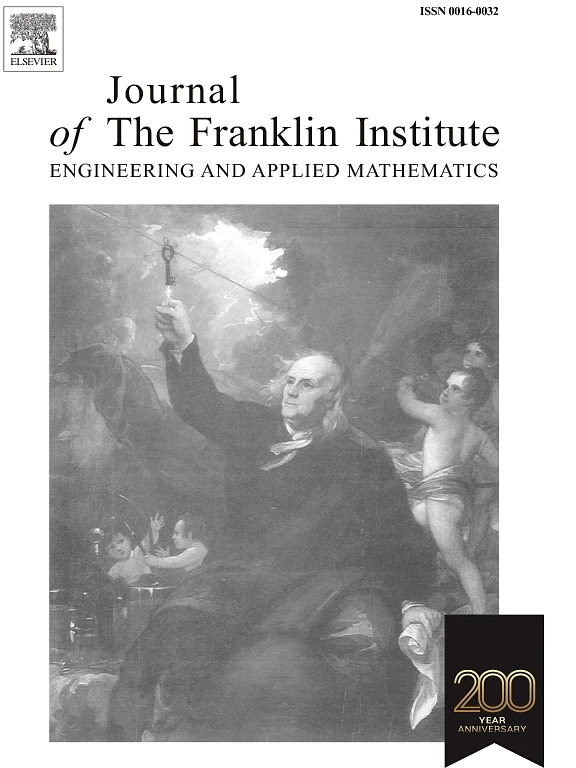
\includegraphics[height=\hb@colwidth, keepaspectratio]{journal-logo}
			} \\
		\end{tabular}
	\end{minipage}
	\par\vskip2pt
	\noindent\textcolor{black}{\rule{\textwidth}{3pt}}
	\par\vskip18pt
}

\let\originalmaketitle\maketitle
\def\maketitle{
	\makeheaderbox
	\vspace{2pt}
	\begin{center}{\Large\bfseries \emph{Bicentennial Special Issue Invited Paper}}
    \end{center}\par
	\vspace{10pt}
	\originalmaketitle
}
\makeatother


%\usepackage[numbers]{natbib}
\usepackage[authoryear,sort]{natbib}
%\usepackage[authoryear,longnamesfirst]{natbib}

%%%Author macros
\def\tsc#1{\csdef{#1}{\textsc{\lowercase{#1}}\xspace}}
\tsc{WGM}
\tsc{QE}
\tsc{EP}
\tsc{PMS}
\tsc{BEC}
\tsc{DE}
%%%

% keep the forced line break in \title out of the PDF-string metadata
\pdfstringdefDisableCommands{\def\\{}}

\begin{document}
\let\WriteBookmarks\relax
\def\floatpagepagefraction{1}
\def\textpagefraction{.001}
\shorttitle{Learning to Compute and Learning to Play}
\shortauthors{X. Xie et~al.}
%\begin{frontmatter}

\title [mode = title]{Learning to Compute and Learning to Play:\\
Strategic Guarantees for AI in Games}

\author[1]{Xiaohan Xie}
\author[2]{Wenxuan Liu}
\author[1]{Junhua Zhao}
\author[3]{Biying Shou}
\author[1]{Jianwei Huang}
\cormark[1]
\ead{jianweihuang@cuhk.edu.cn}

\affiliation[1]{organization={School of Science and Engineering, The Chinese University of Hong Kong, Shenzhen},
                city={Shenzhen},
                country={China}}
\affiliation[2]{organization={School of Electrical and Electronic Engineering, Nanyang Technological University},                 
                country={Singapore}}
\affiliation[3]{organization={Shenzhen Finance Institute, School of Management and Economics, The Chinese University of Hong Kong, Shenzhen},
                city={Shenzhen}, country={China}}

\cortext[cor1]{Corresponding author}

\begin{abstract}
Learning now plays two roles in game theory: it computes strategic solutions, and it
acts as a strategic participant in its own right. In both, a learned strategy, model,
or rule is only a candidate until an argument certifies the property claimed for it. We
organize the field around the two questions that argument must answer---whether a
learned output actually has its claimed strategic property (the \emph{claim question}:
does it hold?), and whether a property proved inside a designed game delivers the
objective the game was built to serve (the \emph{goal question}: does it help?). We
read six domains through these questions, from equilibrium computation to
algorithmic-pricing governance, including deployments where participants' responses
change the cases a rule later meets. Read together they give one answer: learning has
changed which strategic computations are cheap, not what makes a strategic claim true.
\end{abstract}

%\begin{graphicalabstract}
%
\includegraphics{figs/cas-grabs.pdf}
%\end{graphicalabstract}

%\begin{highlights}
%\item Research highlights item 1
%\item Research highlights item 2
%\item Research highlights item 3
%\end{highlights}

\begin{keywords}
learning in games \sep equilibrium computation \sep strategic inference \sep
automated mechanism design \sep strategic evaluation \sep algorithmic pricing
\end{keywords}


\maketitle

% intro.tex
% Section 1: Introduction

\section{Introduction}
\label{sec:intro}

Game theory first asks whether a solution exists. \Citet{Neumann1928} showed that every
finite two-person zero-sum game has a value together with a pair of optimal
mixed strategies, and \citet{vNM1944} incorporated
this result into a general theory of economic behavior. \citet{Nash1951}
extended equilibrium existence to finite games with any finite number of players
and general payoff interactions, well beyond strictly
competitive play.

Mechanism design asks how the rules of interaction should be chosen. In
the standard quasilinear setting, the Vickrey--Clarke--Groves family showed how
to make truthful reporting a dominant strategy by charging each participant for
the externality it imposes~\citep{Vickrey1961,Clarke1971,Groves1973}, and
\citet{Myerson1981} characterized the
revenue-maximizing auction for the single-item Bayesian
setting. Impossibility results identify combinations of
domain restrictions and desiderata that cannot be satisfied
simultaneously~\citep{Arrow1951,Gibbard1973,Satterthwaite1975}.
Together, such results frame mechanism design as the selection of rules under
explicit incentive and feasibility constraints.

Once a solution concept has been defined and its existence established, the
next question is how to compute a solution. Algorithmic game theory studies
this question for different game representations and solution concepts
~\mbox{\citep{NisanRoughgardenTardosVazirani2007}}. Computing a Nash
equilibrium is PPAD-complete in general, and remains so with only two
players~\citep{DaskalakisGoldbergPapadimitriou2009,ChenDengTeng2009}. Even
classical constructive procedures can follow exponentially long
paths~\citep{LemkeHowson1964,SavaniVonStengel2006}. Established approaches weaken
the solution concept or exploit a restricted game's structure, often while
accepting approximation.

\subsection{How Learning Changes Computation}
\label{sec:intro:change}

Learning can amortize computation across related instances. An amortized method
trains a conditional rule on a family of related cases and reuses that rule on
new cases. This is the standard setup in amortized optimization and
inference~\citep{Amos2022Amortized,KingmaWelling2014}, and it has also been used
in strategic systems. In heads-up no-limit poker, learned counterfactual values
and continual re-solving are among the methods that have produced expert-level
play~\citep{Moravcik2017,BrownSandholm2018,BrownReBeL2020}. Self-play with
learned policy and value networks mastered board games from their rules, and
league training produced a StarCraft II agent at grandmaster
level~\citep{Silver2018,Vinyals2019}. Neural networks now also search spaces of
auction mechanisms that no analyst could
enumerate~\citep{Duetting2019,Duan2023,Duetting2024}.

In these examples, learning is used as part of the solver: training shares
computation across related instances and can reduce the cost of solving later
ones. A learned system can also participate in the interaction being studied.
Pricing algorithms operate in real
markets~\citep{Calvano2020,Assad2024}. Language models negotiate and
coordinate~\citep{Bianchi2024NegotiationArena,Akata2025}, while preference-based
training procedures use human feedback on model outputs to train policies,
often via learned reward models~\citep{Christiano2017,Ouyang2022}.
In each case the system's outputs can change what other participants do and
which situations the system later faces. Performance on a fixed set of cases
does not by itself establish performance after those responses. Game-theoretic
deviation tests provide one relevant standard: whether a participant can gain
by deviating within a specified class.

\subsection{Construction and Validity}
\label{sec:intro:cost}

Evidence for learning-based strategic methods typically comes from finite
searches or test populations. RegretNet reports the largest gain found by
gradient search over sampled valuation profiles~\citep{Duetting2019}. Poker
systems report performance against a test population
~\citep{Moravcik2017,BrownSandholm2018,BrownReBeL2020}, while pricing audits
estimate regret against alternatives recoverable from deployment
logs~\citep{HartlineLongZhang2024}. Each result provides evidence for sampled
cases and accessible alternatives. Some target properties are defined over a
broader deviation class than the evaluation covers. For example, they require
that no deviation in the specified class be
profitable or that truthful reporting yield at least as much utility as every
admissible misreport for every type. For such deviation-defined properties, one
profitable deviation refutes the claim. A search that finds no profitable
deviation supports a claim over the full target class only if it covers that
class, or if a separate argument bounds the gain available from deviations
outside the search space.

We distinguish two forms of validity.

\begin{description}
\item[Output validity.] Does the learned output have the claimed strategic
property? The answer depends on how the game and candidate can be queried or
checked.

\item[System validity.] Does a property established inside a designed game
support the objective that the game was designed to serve? For an alignment procedure, oversight protocol,
or market institution, this depends on how the designed interaction represents
both the participants and the objective.
\end{description}

The available access determines what further argument is possible. When each
alternative can be evaluated through an explicit model or simulator, the main
obstacle may be the size of the class. We call this a coverage limit. Broader
search or a bound derived from structure may address it.
With observational data, distinct strategic models can instead generate the
same realized behavior. This identification limit cannot be resolved by more
data from the same observational regime. It requires informative variation,
intervention, or maintained restrictions~\citep{HaileHortacsuKosenok2008}.
Figure~\ref{fig:validity-gates} summarizes these two validity questions and the
implication that must hold in each case.

\begin{figure}
\centering
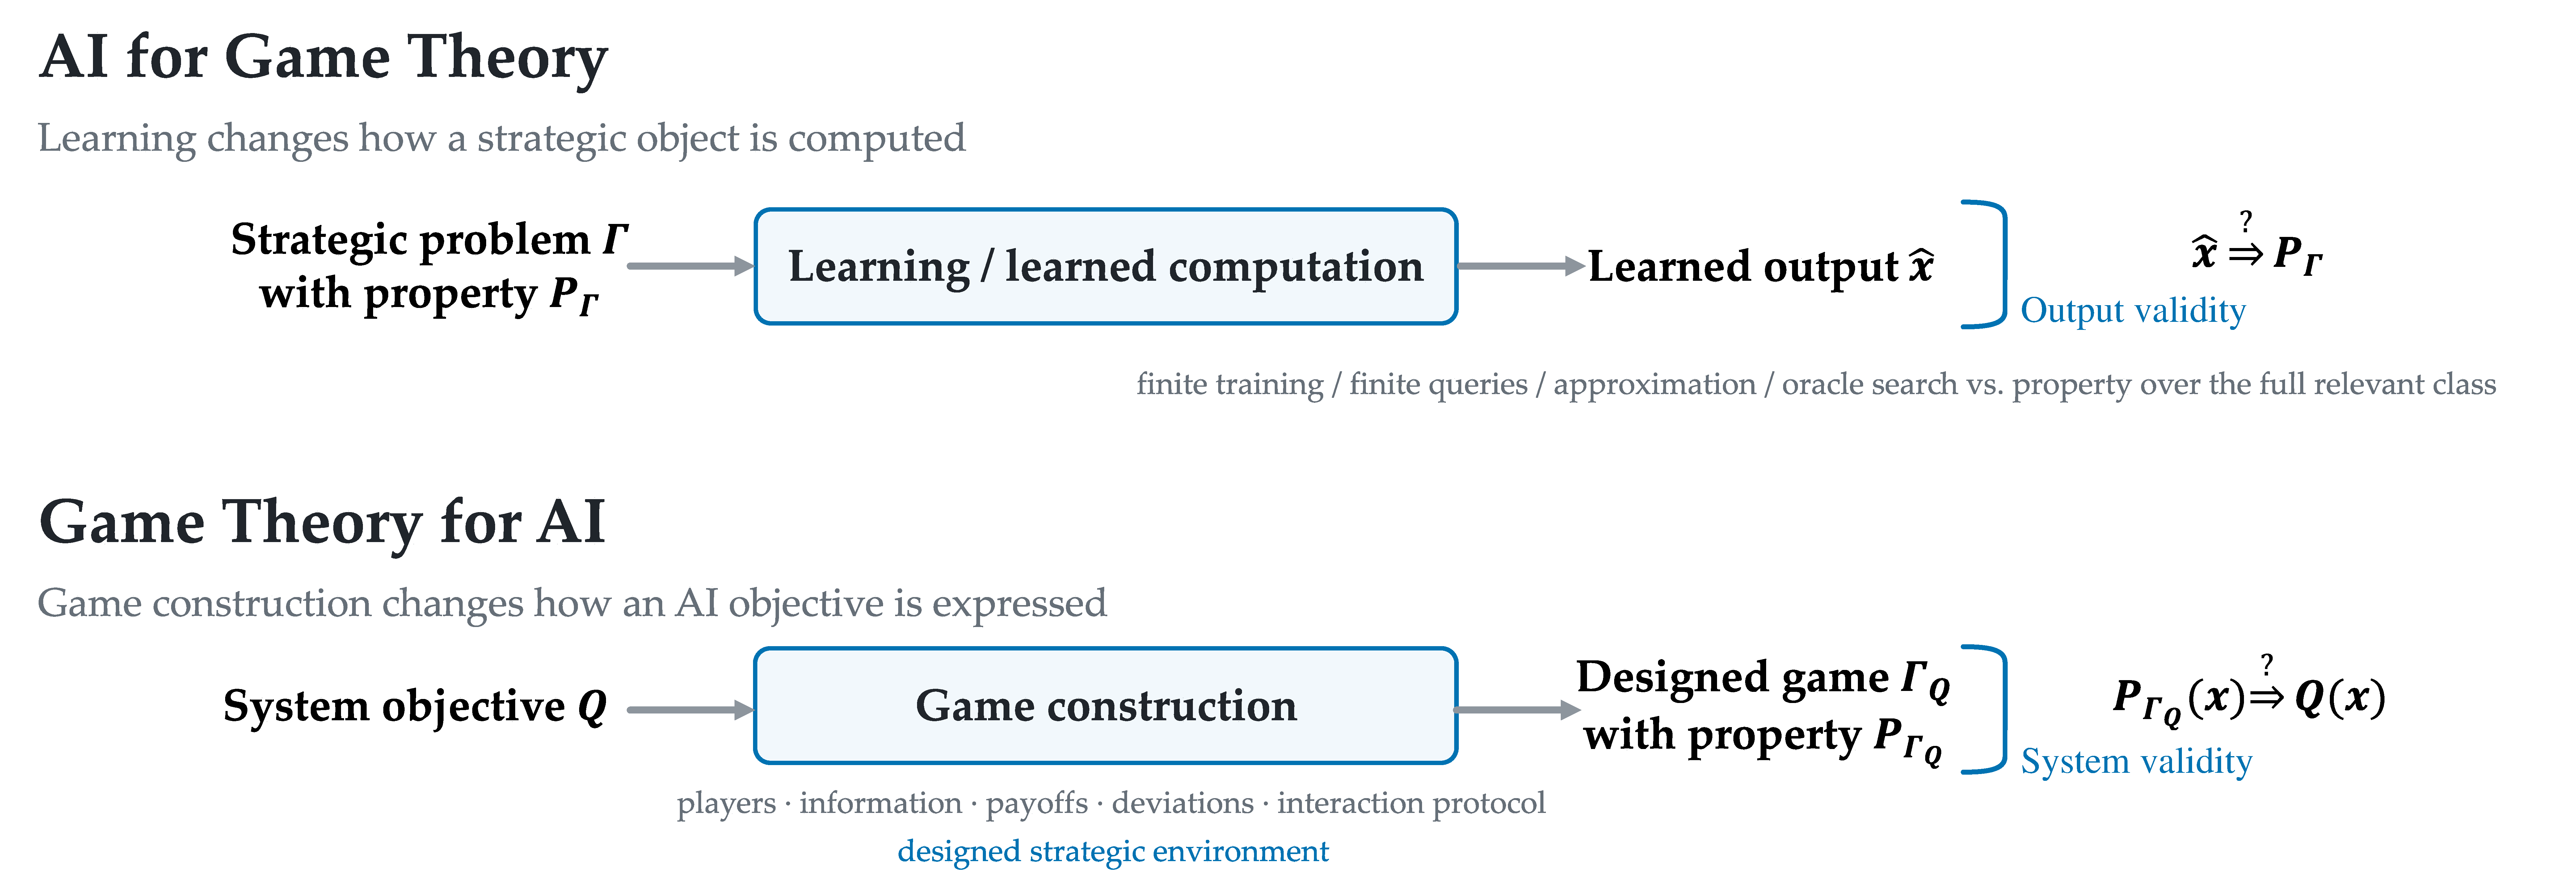
\includegraphics[width=\textwidth]{figure/fig1-preservation-gaps.pdf}
\caption{The two validity questions. \emph{Output validity} concerns the
strategic property of a learned output. \emph{System validity} concerns whether
a property established inside a designed game supports the game's external
objective. Section~\ref{sec:synthesis} gives the conditions for composing the
two implications.}
\label{fig:validity-gates}
\end{figure}

\subsection{Why the Distinction Matters}
\label{sec:intro:why}

The distinction matters when learned strategic systems are evaluated beyond a
fixed benchmark. Field evidence from retail gasoline markets links algorithmic
pricing to higher margins~\citep{Assad2024}. In oligopoly experiments,
language-model agents reach supra-competitive prices without
instruction~\citep{FishGonczarowskiShorrer2024}. Language models also propose
executable mechanisms and equilibrium derivations
~\citep{PrimeNash2025,LegoNE2025,LiuGuoConitzer2025}. These outputs can be
checked mechanically against a formal specification. Executability alone does
not supply that specification or establish the strategic claim.

The same evidentiary question appears in proposals to regulate algorithmic
collusion. These proposals ask whether a firm can produce evidence that its
pricing algorithm was not exploiting its rivals, with the burden of producing
that evidence assigned by
rule~\citep{HartlineLongZhang2024,HartlineWangZhang2025,Harrington2018}. When a
statistical property of a deployment log is offered as a legal defense, the
scope of the claim supported by that finite evidence becomes part of the
proposed regulatory design.

\subsection{Scope and How to Read This Survey}
\label{sec:intro:scope}

\paragraph{Scope.} We study systems that learn strategic rules from data or
interaction. A high-dimensional trained rule may require empirical queries
and statistical bounds, whereas executable code or membership in a structured
family may permit direct checking. The appropriate analysis therefore depends
on the representation and the property being claimed.

\paragraph{Related surveys and exclusions.} Stackelberg
and security games, mean-field games, multi-agent reinforcement learning beyond
its use as a response oracle, autobidding, and incentive design for federated
learning fall outside our selected domains. \citet{WellmanTuylsGreenwald2025}
and \citet{CurryAMDSurvey2025} provide focused reviews of empirical
game-theoretic analysis and automated mechanism design, respectively.
\citet{SunWuChengChu2025} survey the game theory--LLM intersection with the
language model as the focal technology. \citet{Podimata2025} surveys
incentive-aware machine learning, where individuals adapt their inputs to a
deployed decision rule. Each of these surveys organizes the literature around
its object of study. We organize by the relation between a computation, the claim attached
to it, and the evidence available for that claim.

\paragraph{Organization.} Section~\ref{sec:recap} introduces the computational
background. Sections~\ref{sec:ai4gt} and~\ref{sec:gt4ai} organize six application
areas around the two validity questions, as illustrated in
Figure~\ref{fig:survey-route}. Section~\ref{sec:synthesis} states when the two
can be combined. After deployment, participants' responses can alter the inputs
and counterparties that the system encounters. Performative prediction
provides one formalization of such feedback~\citep{Perdomo2020Performative}. A
guarantee established on a fixed evaluation distribution need not extend to the
deployment distribution shaped by those responses. The relevant response
process and case domain must therefore be specified as part of the claim.

\begin{figure}[pos=ht]
\centering
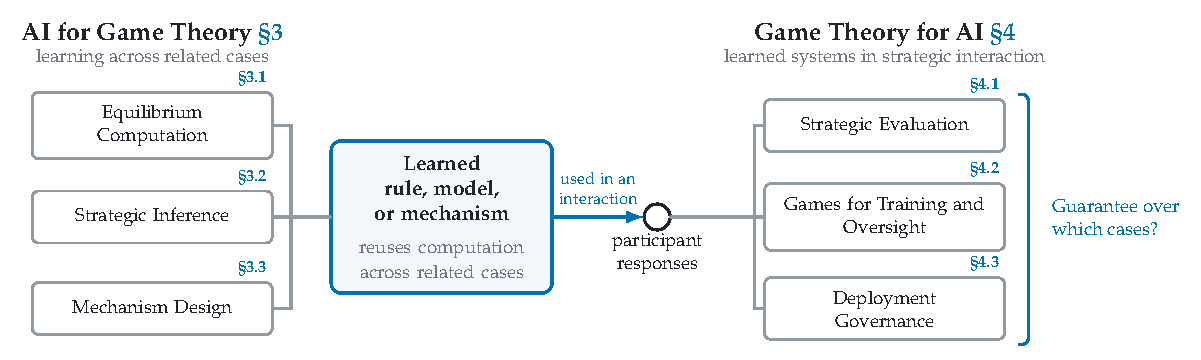
\includegraphics[width=0.9\textwidth]{figure/fig2-survey-route.pdf}
\caption{Survey structure and the interaction link. Section~3 studies learned
strategic objects across related cases. Section~4 studies learned systems in
interactions where participant responses can change the relevant cases. The
six labels identify the corresponding subsections and need not be disjoint.}
\label{fig:survey-route}
\end{figure}

\FloatBarrier

% recap.tex
% Section 2: Background

\section{Background}
\label{sec:recap}

Equilibrium and incentive compatibility are both defined by deviations.
Computing an equilibrium, or verifying incentive compatibility for a candidate
mechanism, can be costly. Learning can share computation across related
instances, but it does not itself establish the relevant guarantee. A learned
output therefore still needs a check or bound specific to the claimed property.

\subsection{Equilibrium Conditions and Computational Demands}
\label{subsec:recap-gt}

For both concepts, the relevant deviation class determines what must be checked.
We first state the corresponding deviation conditions, then separate
constructing a candidate from verifying it. The final subsection reviews
standard restrictions and relaxations that recover tractability.

\subsubsection{Equilibrium and its deviation class}

Von Neumann's minimax theorem establishes that every finite two-player zero-sum
game has a value and a pair of optimal mixed
strategies~\cite{Neumann1928,vNM1944}. In that setting a player's equilibrium
strategy is also its worst-case-optimal strategy, so equilibrium and robustness
coincide. This coincidence is specific to strictly competitive play and does not
extend to general games.

Nash's equilibrium is a profile in which no player gains by deviating
alone~\cite{Nash1951}. The condition can be quantified through each player's
best unilateral gain. For a profile $s$ and a class $\mathcal{D}_i$ of
deviations available to player $i$, write the aggregate gap
\[
  \mathrm{Gap}_{\mathcal{D}}(s)
  \;=\;
  \sum_i \Bigl[\, \sup_{s_i' \in \mathcal{D}_i} u_i(s_i', s_{-i}) - u_i(s) \,\Bigr].
\]
Assume that $\mathcal{D}_i$ includes the player's current strategy. When each
$\mathcal{D}_i$ is the player's whole strategy set, this sum is commonly called
NashConv; closely related normalizations are called exploitability. It is zero
exactly at a Nash equilibrium. In other applications $\mathcal{D}_i$ may be a
restricted class, in which case the gap describes only deviations in that class.

The deviation inequalities can be evaluated one player at a time while holding
the opponents' strategies fixed, but every player's inequality must hold for
the same joint profile. The condition is static and does not describe whether an
adaptive process reaches such a profile. That requires a convergence analysis of
the process itself.

Extensive-form games represent the order of play and the information available
to each player, and Kuhn's
theorem established that under perfect recall mixed and behavioral strategies
induce the same outcome distributions~\cite{Kuhn1953}. Selten's refinements
imposed rationality at contingencies the equilibrium path never
reaches~\cite{Selten1975}. Harsanyi handled private information by making a
player's payoff-relevant characteristics a \emph{type}, converting incomplete
information into a Bayesian game~\cite{Harsanyi1968}. In each case the
comparison with counterfactual alternatives remains the content of the concept,
with the refinements changing the set of alternatives being compared.

In a correlated equilibrium, a mediator draws a joint action profile and
privately recommends one action to each player. No player gains by deviating as
a function of the recommendation received~\cite{Aumann1974}. Quantal response
equilibrium replaces exact best response with a smooth choice rule in which
better actions are more likely, but mistakes persist~\cite{McKelveyPalfrey1995}.

\subsubsection{Design and deviation-based incentive constraints}

Mechanism design chooses rules under which participants' incentives produce a
desired outcome.
Impossibility results identify restrictions on what particular classes of
rules can achieve~\cite{Arrow1951,Gibbard1973,Satterthwaite1975}. Under the
conditions of the revelation principle, the design problem can be posed over
direct mechanisms in which agents report types and truthful reporting is an
equilibrium.

Incentive compatibility is likewise defined by deviations: for every relevant
type, truthful reporting must do at least as well as \emph{every} admissible
alternative report. Here the deviation class is the misreport space, with its
scope determined by the equilibrium concept and the mechanism's domain. The
Vickrey--Clarke--Groves family achieves efficient allocation in dominant
strategies~\cite{Vickrey1961,Clarke1971,Groves1973}, and Myerson characterized
the revenue-optimal single-item Bayesian
auction~\cite{Myerson1981}.

\subsubsection{Construction and checking}

The PPAD-completeness results noted at the start of the introduction concern
total search problems: a solution exists, although finding one may be
intractable~\cite{Papadimitriou1994}. The asymmetry between construction and
checking also depends on the representation and the property. Given an explicit finite game and a rational profile,
evaluating a specified deviation is direct. Finding one profitable deviation
refutes the equilibrium claim. Establishing that no profitable deviation exists
over a large or implicitly represented class can require an optimization or
structural result. Mechanism design faces the
same computational pressure because optimization over contingent rules is
itself a hard search problem~\cite{ConitzerSandholm2002}.

\subsubsection{Standard routes to tractability}

Tractability can be recovered by weakening the solution concept or restricting
the game class, often while accepting a bounded residual gain. For example, correlated
and coarse correlated equilibria in explicitly represented finite games admit
linear descriptions and are computable in polynomial time. They can also arise
from decentralized learning: when every player in a repeated game
drives external regret to zero, the empirical distribution of play approaches
the coarse correlated set, and stronger regret notions reach the correlated
set~\cite{Hannan1957,HartMasColell2000,BlumMansour2007}. The deviation class is
explicit in this result: the equilibrium notion obtained depends on which
deviations the regret criterion compares against~\cite{GordonGreenwaldMarks2008}.
Each modification changes the claim for which a deductive guarantee is
available. Learning can be combined with any of them by fitting a conditional
rule across related games and reusing it on later instances.

\subsection{What Training Does}
\label{subsec:recap-dl}

Section~\ref{subsec:recap-dl} first explains how training amortizes computation
across instances, then turns to training cost and the guarantees that must still
be established after training.

\subsubsection{Amortization: sharing computation across instances}

A per-instance solver is invoked on a specified game. An amortized system fits
a conditional rule across a family of related cases and later evaluates that
rule on a new case. Total computation includes training and later evaluations.
The potential advantage comes from sharing the trained rule across cases. This
is the structure of amortized optimization and
inference~\cite{Amos2022Amortized,KingmaWelling2014}. Different architectures
encode different forms of sharing across states or instances.

Reinforcement learning adds the dependence that matters for strategic settings:
an action changes the data the learner will next
observe~\cite{SuttonBarto2018,Williams1992,SuttonPolicyGradient2000,Mnih2015}.
When the rules are known, self-play can generate new training games as the
policy changes, an approach used to train policy and value networks in board-game
systems~\cite{Silver2018}. When behavior is observed
but the objective is hidden, inverse reinforcement learning estimates which
objectives are consistent with that behavior~\cite{NgRussell2000,HoErmon2016}.

Preference-based fine-tuning turns
comparisons between outputs into a training signal, making the learning target
itself something another party
supplies~\cite{Christiano2017,Ouyang2022}. Large language models generate
general-purpose text~\cite{BrownGPT3_2020}. Code models and tool-using agents
also produce executable programs or action traces
~\cite{ChenCodex2021,YaoReAct2023,SchickToolformer2023}.

\subsubsection{What must still be accounted for}

Amortization changes where the computation occurs. Data generation and parameter
optimization can dominate the time saved at inference, so a cost comparison
should include training as well as later evaluations. The strategic property of
the output then depends on the analytic or post-training check used by the
method.

Validation also depends on access. A high-dimensional rule may be available only
through queries, and finite tests cover sampled instances and representable
alternatives. Extending such results to a larger deviation class requires a bound
or structural argument. Executable code and rules constrained to a known family
may instead permit symbolic checking or a direct theorem.

Construction and validation impose separate costs. Learning can amortize
construction across related instances, but it does not by itself establish the
target property over the full deviation class. Sections~\ref{sec:ai4gt}
and~\ref{sec:gt4ai} identify the additional argument required in each
application domain.

\section{Learning to Compute Strategic Solutions}
\label{sec:ai4gt}

When can the evidence in hand support a game-theoretic property claimed for a learned output, the \emph{claim question} (does it hold?) of
Section~\ref{sec:intro}? The answer depends on what the learner had access to, and
that access differs sharply across three settings. An equilibrium solver usually
starts from an explicit game or simulator, so it can evaluate any individual deviation, even when the full deviation class
is too large to exhaust. Strategic inference has less to work with: it observes play generated by
an unknown game, and different latent games can explain the same play equally
well. A learned mechanism is in between. It can be queried on types and misreports
before deployment, but publishing it can change who participates and
what they report afterward. Figure~\ref{fig:claim-obstacles} contrasts two recurring obstacles
that organize much of this section. Under
\emph{coverage}, the searched class is only part of the full
one, and a bound or more search must cover the rest. Under
\emph{identification}, distinct latent models fit the same play, and more data
cannot separate them. Throughout, the learned component supplies a candidate; what
certifies the property claimed for it is the surrounding argument, not the
learning. The rest of this section takes the three settings in
turn.

\begin{figure}[pos=t]
\centering
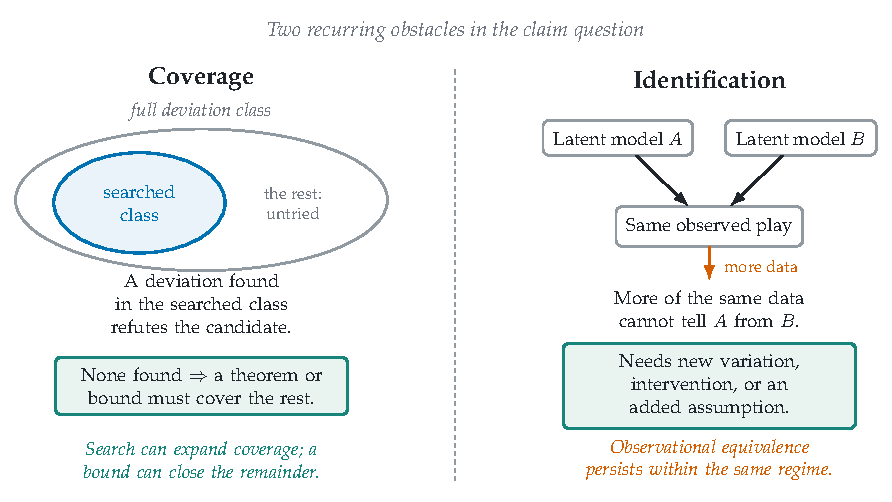
\includegraphics[width=\textwidth]{figure/fig5-claim-obstacles.pdf}
\caption{Two recurring obstacles in the claim question. \emph{Left (coverage):} the class
actually searched is a subset of the full deviation class; a deviation found there
refutes the candidate, but ruling out the rest needs a theorem or bound.
\emph{Right (identification):} two latent models can produce the same observed play,
and more of the same data cannot tell them apart --- only new variation,
intervention, or an added assumption can. Coverage recurs in equilibrium computation
(\S\ref{sec:ai4gt:equilibrium}), mechanism design (\S\ref{sec:ai4gt:mechanism}), and
strategic evaluation (\S\ref{sec:gt4ai:evaluation}); identification governs strategic
inference (\S\ref{sec:ai4gt:inference}) and joins coverage in deployment governance
(\S\ref{sec:gt4ai:governance}).}
\label{fig:claim-obstacles}
\end{figure}

\subsection{Equilibrium Computation with Learning}
\label{sec:ai4gt:equilibrium}

Take a solver computing a poker strategy. It can evaluate any specified bluff, but
the condition it must certify --- that \emph{no}
deviation pays --- ranges over the whole deviation class, far more than it can try.
That gap is the central tension of this subsection. Learned methods answer it by
pairing finite search with problem-specific analysis that controls what the search
left out; absent that analysis, the residual is measured only over the deviations
actually tried. We start from the classical baseline,
then cover learned quantities inside a solver, learned responses and
continuation values, and finally symbolic proposals that admit a direct check.

\subsubsection{Complexity and classical baseline}
The hardness results from the introduction apply to general finite games, but not
uniformly. Two-player zero-sum games (poker among them) occupy an easier regime, because their equilibrium conditions can be written as a matched pair of
linear programs, one per player. No-regret dynamics give a second route in: if two
players each drive their regret to zero, their average strategies approach the
minimax solution. This regret-to-equilibrium link is what the poker solvers later in
this subsection rely on, and it is special to two-player zero-sum play: it does not carry over unchanged to
general-sum games.

Classical numerical methods set the reference point. A fixed algorithm is already
reusable across explicitly represented games, though its computation is not
adapted from any training distribution. In a finite bimatrix game, support enumeration searches over possible supports
and solves the associated indifference and inequality conditions. The
Lemke--Howson algorithm recasts equilibrium as a linear complementarity
problem and pivots along a complementary path to a fully labeled
solution~\citep{LemkeHowson1964}. Homotopy methods embed the game in a
parameterized family and follow an equilibrium path from an easier auxiliary
problem. Gambit implements several of these
representations and algorithms~\citep{gambit}. All of them require finite, fully
represented games, and their worst-case cost stays substantial: Lemke--Howson can follow an
exponentially long path~\citep{SavaniVonStengel2006}.

\subsubsection{Learned quantities within equilibrium procedures}
When learning enters from inside the solver, it replaces a computed quantity ---
a response map, a value, a regret --- with a learned one. Each
method is therefore best assessed by the surrounding analysis: what it proves, for
which class of games, and to what target. Three sources of guarantee recur --- a direct
convergence proof, a regret bound, or, failing both, only empirical strength ---
and the target that can be certified weakens as the games leave the two-player
zero-sum case. Figure~\ref{fig:learning-substitution} lays out the three.

\begin{figure}[pos=t]
\centering
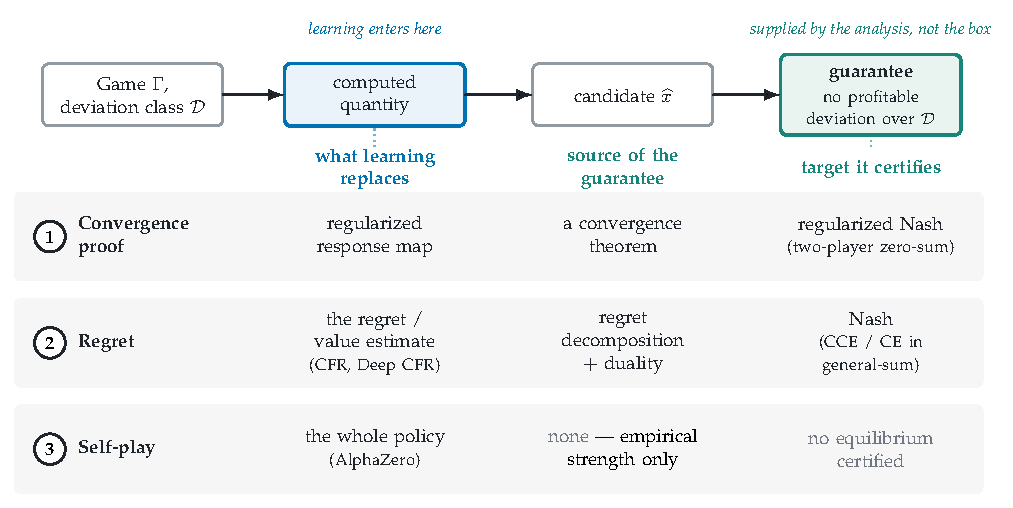
\includegraphics[width=\textwidth]{figure/fig3-learning-substitution.pdf}
\caption{Learning inside the equilibrium solver, and where the guarantee comes from.
The top row is the general shape of the claim question (cf.\
Figure~\ref{fig:claim-obstacles}): a learned quantity enters the solver, while a
separate convergence analysis, regret bound, or empirical evaluation determines
what can be claimed about the output. The three rows identify the learned
replacement, the supporting analysis, and the resulting target.
(Section~\ref{sec:ai4gt:equilibrium})}
\label{fig:learning-substitution}
\end{figure}

\runin{Guarantee from a convergence proof.} The first route smooths the response map, making it differentiable and therefore
amenable to policy-gradient and neural optimization. This smoothing, however,
shifts the target: any resulting guarantee applies to a regularized equilibrium
rather than the original equilibrium. \citet{NashPG2025} establish the strongest
such result. For an idealized refinement procedure, they prove that every step
strictly reduces the Bregman divergence to any Nash equilibrium and that the
procedure converges in two-player zero-sum extensive-form games. Yet this guarantee
applies to the idealized procedure, not to NashPG, the sampled algorithm used in
practice. \citet{LiuFarinaOzdaglar2025} expose the same limitation from another
angle by proving best-iterate convergence to a regularized equilibrium. Their result concerns only the best iterate (not every subsequent policy) and
only the regularized target. In both cases, the proof is substantive, but what it certifies
is narrower than the practical method built upon it.

\runin{Guarantee from regret.} The second route requires less machinery. Rather than proving convergence
directly, it derives the guarantee from regret. Once a learner's average regret
vanishes, no fixed deviation retains a persistent advantage in hindsight. In a
two-player zero-sum game, duality converts this into a bound on the exploitability
of the average strategy. Counterfactual regret minimization (CFR) extends the idea
to extensive-form games by decomposing the overall regret across information
sets~\citep{Zinkevich2007}. It is this decomposition, rather than a separate
argument, that yields the exploitability bound.

This guarantee is exact but tabular. Scaling it beyond an explicit table degrades
it, though in a controlled manner. Deep CFR replaces the tabular regrets with
neural approximations~\citep{BrownDeepCFR2019}, so that sampling and
function-approximation error enter the same exploitability bound through the same
regret decomposition. The guarantee is therefore not lost but widened, by an error
term the analysis makes explicit.

\runin{No equilibrium guarantee: self-play.} Return-maximizing self-play without an
equilibrium-residual objective offers no equilibrium guarantee from training alone.
It can achieve strong play, as AlphaZero shows, without ever minimizing an
equilibrium residual. It provides empirical evidence of performance against the
training population, which may hide a profitable counterstrategy or permit
cycling among mutually exploitable policies. Methods that do certify an equilibrium
require an analysis connecting the training objective or stopping rule to the stated
target, for example through a controlled equilibrium residual or response-oracle
condition.

Every route so far has assumed two-player zero-sum play, where the target is
unambiguous. In general-sum games it is not, and the certifiable guarantee weakens
accordingly. Independent external-regret minimization now reaches only the coarse
correlated equilibria (CCE); stronger internal- or swap-regret guarantees reach
the correlated equilibria (CE). The two differ by deviation class: a coarse
correlated equilibrium rules out committing to a fixed action before observing a
recommendation, whereas a correlated equilibrium also rules out deviations that
condition on it. Both are weaker than Nash equilibrium, since neither requires the
joint distribution to factorize into independent strategies. The weaker target is
also computationally cheaper: these equilibria admit linear descriptions and are
verifiable in polynomial time. It remains, however, a different target, since
reaching a coarse correlated equilibrium does not solve the original Nash problem.
Meta-learned CFR treats this residual gap as its objective, training a
parameterized regret minimizer whose meta-loss measures the distance remaining to
the stronger Nash condition~\citep{Sychrovsky2025}.

\subsubsection{Learned responses for empirical games}
The previous route assumed the solver could work with the game itself: evaluate deviations, form regrets,
invoke duality. That assumption breaks when the game is
given only by a simulator, its normal form too large to enumerate. Empirical
game-theoretic analysis proceeds anyway. It approximates the game by a finite policy
population: the analyst picks a strategy set, estimates its payoffs by simulation,
and solves the resulting empirical game~\citep{WellmanTuylsGreenwald2025}. The
guarantee question shifts with the setting. It is no longer whether an analysis
certifies a learned quantity, but whether the population covers the deviations that
matter. The methods below are two ways of growing and solving that population, each
leaving its own coverage gap.

\runin{Response-oracle expansion.} Policy-space response oracles (PSRO) grow the
population adaptively~\citep{Lanctot2017}. They solve the current empirical game,
train an approximate best response to its meta-strategy, add that policy, and
estimate the new payoff entries. A multi-agent reinforcement learner supplies the
response oracle; the empirical-game solver coordinates the policies already found.
Pipeline PSRO runs several such response processes and empirical-game updates
concurrently for scale~\citep{McAleerPipelinePSRO2020}. What the population certifies
is only as strong as the responses the oracle can find.

\runin{Correlated-equilibrium meta-solvers.} Joint policy-space response oracles
(JPSRO) keep the population structure but change the solution concept used for the
empirical game~\citep{Marris2021}. At each iteration a deep reinforcement-learning oracle
searches for responses to a distribution drawn from the empirical game. Max-Gini
selection then picks a high-entropy correlated or coarse correlated equilibrium
among the solutions. The output is a CE or CCE of the empirical game: the same retreat to a weaker
target seen for general-sum games above, now driving population
growth rather than relaxing a regret bound.

Carrying any of these solutions back to the underlying game requires accurate payoff
estimates and coverage of deviations outside the current population. Here the finite
empirical game is not one ingredient of the solver but an approximation standing in
for the underlying game, and the quality of that approximation sets what the solution
supports.

\subsubsection{Learned continuation values for online re-solving}
The last two routes changed what the computation runs on: shared across
instances, or a population standing in for the game. This route keeps the game exact
and changes instead \emph{when} the computation runs. Large imperfect-information
games can postpone work until play reaches a subgame. A solver builds a coarse
blueprint offline and re-solves the current subgame online, which injects extra
exploitability at the subgame boundary. What holds that error in check is the
organizing question, and the answer tracks how much of the continuation is learned
rather than computed exactly. Three systems span the range.

\runin{Bounded learned values.} DeepStack keeps the continuation learned and bounds
the resulting error~\citep{Moravcik2017}. In heads-up no-limit poker it continually
re-solves the public portion of the game, calling a neural counterfactual-value
function beyond a limited lookahead. The network thus compresses continuation
computation across public states, while continual re-solving and
counterfactual-value bounds hold the added exploitability in check. The learned
value is what is deferred; the bound is what certifies it.

\runin{Exact safe re-solving.} Libratus reaches the same end with no learned value
at all~\citep{BrownSandholm2018}. It combines a CFR-based blueprint with nested safe
subgame solving and endgame refinement, its safe-resolving component carrying no
neural approximation. This marks the exact end of the range: the boundary
exploitability is controlled by construction, not by a bound on a learned object.
That control is precisely what DeepStack's value network trades away for scale.

\runin{Reformulation with a convergence proof.} ReBeL neither bounds a learned value
nor forgoes learning; it reformulates the game so that a proof becomes
available~\citep{BrownReBeL2020}. Each public belief state pairs public information
with a distribution over the players' private states. This yields a
continuous-state, perfect-information game on which reinforcement learning and
search can operate. Trained through self-play as policy and value networks, ReBeL is
used inside nested subgame solving. For two-player zero-sum games, it admits a proof
of convergence to Nash equilibrium under the prescribed representation and solving
assumptions. Private information stays hidden: the public belief state is all the
recursion needs.

Across the range, the boundary guarantee comes from the re-solving analysis --- a
value bound, a safe-resolving construction, or a convergence proof --- not from the
learned value alone. Figure~\ref{fig:learning-substitution} draws the same
separation for the equilibrium pipeline. What moves along the range is only how much
of the continuation is entrusted to learning.

\subsubsection{Symbolic proposals under executable checks}
The routes so far attached a guarantee to a learned numerical object --- a value, a
regret, a response --- and bounded its error. This route breaks that dependence. A generator proposes a symbolic object (an equation, or code) for an
individual game, and a separate formal or computational component checks feasibility and the
relevant deviation conditions. Provided the encoding and checker are sound, the
mechanical test establishes the property whatever produced the proposal. That is
what makes an unreliable generator, such as a language model, tolerable. The two
methods below differ only in the level of the generated object: a solution, or the
algorithm that produces one.

\runin{Generating a solution.} PrimeNash targets analytical equilibrium
characterization for an individual game~\citep{PrimeNash2025}. Its agents generate
candidate strategies and symbolic derivations, then call executable tools to
manipulate and test the expressions. The target is an instance-specific symbolic
characterization, parameter regions and boundary cases included. The guarantee
comes from explicit best-response conditions and machine-executable checks, not
from the generator.

\runin{Generating an algorithm.} LegoNE moves the generation one level up, to the
synthesis of equilibrium algorithms~\citep{LegoNE2025}. Expert proof strategies
live in a domain-specific language. Each generated algorithm is compiled into a
finite constrained optimization problem, whose solution determines a worst-case
approximation guarantee for the encoded game class and objective. The check is now
a bound on the algorithm, not a test of one solution.

Across the four learned routes, the guarantee comes from elsewhere than the
learning. Where it is deductive, it rests on the
surrounding analysis: duality, regret decomposition, safe resolving, or verified
constrained optimization. Where it is not, as in empirical games, the claim is only
as strong as the population's coverage. Total cost includes data generation and
training, and any residual approximation should be reported as exploitability or
regret.

\subsection{Strategic Inference: What Observed Play Can Identify}
\label{sec:ai4gt:inference}

The previous subsection ran the pipeline forward: a known game in, a
certified strategy out, the obstacle one of coverage that more search can close.
Strategic inference runs it backward. Watching only realized play (a bidder's bids, or players' moves), it must
recover the game that produced them, with no game
given in advance. Its obstacle is different in kind. Two different valuations can
explain the same bids equally well, and more data from the same auction cannot tell
them apart. This is an identification limit, not a
coverage one: it yields to informative variation or maintained restrictions, never
to sample size alone.

Two questions must be settled in order, and either can fail. The first is
falsifiability: could \emph{any} data prove the model wrong? Often not.
\citet{HaileHortacsuKosenok2008} show that QRE is so flexible that it can fit
any pattern of behavior in a single game. QRE is the model in which players
usually choose better actions but sometimes err, and the result survives even
under strong restrictions on the unobserved noise. A model that fits any observation
has no testable implication on its own: QRE acquires identifying content only when
further assumptions are added, such as a
response rule that stays fixed as the game changes.

The second question is recoverability: granting a falsifiable model, is the latent
quantity pinned to a point? Often it is not. In multi-agent inverse reinforcement
learning, one observed equilibrium is usually consistent with many reward functions.
For the entropy-regularized class they study, \citet{FreihautRamponi2025} show that
a given reward induces a unique quantal response equilibrium. This removes the
equilibrium-selection ambiguity but does not collapse the feasible reward set to a
point. What remains is an identified set, its width recording the leftover
ambiguity. Only informative variation narrows it: cross-game or within-participant
variation can separate explanations that coincide along a single realized path. The
model restrictions decide which differences would be informative, and the data must
actually contain them.

Against this backdrop, learned methods differ mainly in where they insert the
assumption that makes identification possible. Three groups do so at three places:
in a learned response model, in a fixed one, or in a search over candidate models.
Table~\ref{tab:inference_methods} sets the three side by side.

\begin{table}[pos=t]
\centering
\caption{Where learned strategic-inference methods insert the assumption that makes
identification possible. (Section~\ref{sec:ai4gt:inference})}
\label{tab:inference_methods}
\footnotesize
\setlength{\tabcolsep}{3.5pt}
\renewcommand{\arraystretch}{1.25}

\begin{tabularx}{\textwidth}{
    >{\raggedright\arraybackslash}p{0.15\textwidth}
    >{\raggedright\arraybackslash}p{0.20\textwidth}
    Y
    Y
    Y
}
\toprule
\textbf{Assumption location}
& \textbf{Representative methods}
& \textbf{Identifying assumption}
& \textbf{What it recovers}
& \textbf{Remaining limitation}
\\
\midrule

Learned response model
& GameNet~\citep{Hartford2016}, ElementaryNet~\citep{DEon2026ElementaryNet}, and
cognitive-model pretraining~\citep{Bourgin2019}
& The network's architecture or its pretraining data encodes the behavioral theory
& A predictive response model fit to the observed play
& Matching predictions does not validate the model's internal behavioral
interpretation
\\

\addlinespace

Fixed model, estimated latents
& A differentiable equilibrium layer~\citep{Ling2018}, dominance-based
intervals~\citep{CuiYu2023}, and a generative relation model~\citep{Shum2019}
& A specified game plus restrictions --- dominance, regularization --- on the unknowns
& Payoffs, types, or relations, as a point, a set, or a posterior
& Only as sharp as the restrictions; often an identified set, not a point
\\

\addlinespace

Search over symbolic models
& AutoBM~\citep{AutoBM2026}
& A hypothesis space of models and a held-out fit criterion
& A symbolic model that fits the data
& Models with equal fit stay indistinguishable; the whole compatible set should be
carried forward
\\

\bottomrule
\end{tabularx}
\end{table}

\runin{Learning the response model.} The first group lets the network carry the
behavioral theory. GameNet maps a two-player normal-form payoff matrix to a
distribution over actions~\citep{Hartford2016}. Its architecture is symmetric under
relabeling the actions, with layers meant to capture non-strategic (level-$0$) play
and a few rounds of players responding to one another. ElementaryNet exposes a hidden ambiguity in that
design: GameNet's nominal level-$0$ component can itself express strategic
responses~\citep{DEon2026ElementaryNet}. Replacing it with one formally unable to do
so, then adding explicit higher-level modules, recovers statistically
indistinguishable predictive performance. Matching predictions therefore does not
validate the behavioral interpretation of a model's internal parts. A related strategy instead supplies the theory through the training data,
pretraining on synthetic choices from cognitive models before fine-tuning on human
observations~\citep{Bourgin2019}.

\runin{Estimating latent quantities in a fixed model.} The second group fixes the
response model and estimates the hidden quantities inside it: the payoffs, private types, or
relationships among agents that the model treats as unknown. The output may
be a single estimate, a feasible set, or a full posterior, and the methods differ in
what they can identify. A differentiable regularized-equilibrium layer passes
prediction error back to the game's parameters~\citep{Ling2018}. In auction data,
dominance restrictions turn observed bids into intervals of possible valuations,
which then enter the loss of a learned bidding model~\citep{CuiYu2023}. A generative
model of social relations instead supports Bayesian inference over the latent
relationships~\citep{Shum2019}.

\runin{Searching over symbolic models.} The third group searches the model itself.
AutoBM proposes symbolic response models in natural language and code, compiles and
fits them, and selects by held-out likelihood~\citep{AutoBM2026}. But selection
still depends on observed fit. Models that predict the same observations stay
indistinguishable, so downstream decisions should account for the whole compatible
set, not treat the selected model as identified.

Across the three groups, the identifying power is exactly the assumption inserted
--- a network's inductive bias, a fixed model's structure, or a search's admissible
class --- and none of it is supplied by the data. Where the assumptions leave the
latent quantity underdetermined, what the data support is the identified set, and a
conclusion is trustworthy only if it holds across that whole set.

\subsection{Mechanism Design: Learning Rules under Incentive Constraints}
\label{sec:ai4gt:mechanism}

Consider a learned auction. Unlike strategic inference, which only watches, the
designer can feed the mechanism any bid before deployment and see how it responds; the access strategic inference lacked is restored. Yet the mechanism faces two tests
at once: its incentive properties before deployment, and its performance after. The
first test is unforgiving. Incentive compatibility (IC) requires truthful bidding to
beat every misreport, for every bidder type, including bids that never appeared in the sample. Finite training and evaluation establish that only when a theorem or
bound controls the omitted cases. It helps to separate two senses of ``outside the training
distribution,'' because they are not the same kind of problem:

\begin{itemize}
\item From \emph{sampled truthful type profiles} to the deployment type
distribution. This affects objectives computed in expectation (revenue, welfare) and is the
ordinary generalization problem.
\item From \emph{searched misreports} to all profitable deviations. This affects
the incentive claim itself, and it is not an averaging problem: a single
unexamined misreport that pays is a counterexample, not a tail event.
\end{itemize}

The gap from searched misreports to all profitable deviations is what the incentive
claim turns on. Write
\(u_i(v_i, b_i, b_{-i})\) for the utility of agent \(i\) whose true type is
\(v_i\), who reports \(b_i\), and whose opponents report \(b_{-i}\). The first
argument is the true type; the remaining arguments are the submitted reports.
For a direct mechanism, dominant-strategy incentive compatibility then
requires truthful reporting to dominate every misreport:
\[
u_i(v_i,v_i,b_{-i})
\;\geq\;
u_i(v_i,b_i',b_{-i}),
\]
for all agents \(i\), all types \(v_i\), all alternative reports \(b_i'\), and
all opponent profiles \(b_{-i}\). The condition is counterfactual: it weighs truthful reporting against
alternative reports, including ones that may never
appear in the training data. A single profitable misreport shows the mechanism is
not incentive compatible; establishing that it \emph{is} requires the inequality
to hold over the entire type and misreport spaces.

That asymmetry organizes the methods. During training, an optimizer or misreporter
network can submit alternative reports to the candidate mechanism and score their
utility on sampled types. From there the approaches fork: some minimize the
resulting empirical regret in a flexible mechanism class; others restrict the
representation, or add post-training analysis, to cover the full type and report
spaces. Shared parameters let allocation and payment computations be reused across
type profiles, and the remaining costs come from the representation and from
checking beyond the training sample. The parts below organize the methods by where the incentive claim rests: in explicit
constraints, in the empirical regret from searched violations, or in the mechanism's construction.

\subsubsection{Guarantees from explicit constraints: the classical baseline}

Automated mechanism design provides the computational baseline. In a finite type
space, a designer introduces allocation and payment variables for each reported
type profile and optimizes expected revenue or social welfare. Feasibility,
individual rationality, and incentive compatibility enter as explicit linear or
mixed-integer constraints~\citep{ConitzerSandholm2002,CurryAMDSurvey2025}.

The virtue of the direct formulation is also its limit. The number of allocation
and payment variables grows with the cardinality of the agents' joint type space,
and incentive compatibility adds comparisons between truthful and alternative
reports on top. Continuous types usually force discretization, and the resulting
program enforces the constraints only at the chosen grid points unless a further argument controls behavior between them: finer grids shrink
that error while enlarging the program.

\subsubsection{Guarantees from searched violations: incentive compatibility as a loss}

Neural mechanism design trades the table of type-contingent outcomes for
parameterized allocation and payment functions, and turns incentive compatibility
into a quantity to minimize. Two moves recur: make the regret itself the training
loss, or vary the architecture and objective around that loss.

\runin{Regret as the training loss.} RegretNet is the central instance of the
move~\citep{Duetting2019}. Given a reported valuation profile, one network outputs
an allocation and another the payments. The parameters are trained to maximize
expected revenue while controlling violations of incentive compatibility and
individual rationality. For bidder \(i\), ex-post regret at a valuation profile is
\[
r_i(v)
=
\max_{b_i'}
\left[
u_i(v_i,b_i',v_{-i})
-
u_i(v_i,v_i,v_{-i})
\right].
\]
The mechanism is incentive compatible exactly when this is zero for every bidder at
every valuation profile. RegretNet estimates the maximization through gradient-based
searches over misreports, and folds the resulting regret into an augmented-Lagrangian
objective. The shape is a two-player contest: the mechanism network proposes
allocations and payments, and an inner search returns profitable misreports as both
violation and training signal. ALGNet makes the inner player explicit, replacing the
optimization with a learned misreporter~\citep{Rahme2021Auction}. It evaluates regret
over the deviations that misreporter can represent and find. The auctioneer changes
the mechanism to raise revenue; the misreporter searches for reports that raise an
agent's utility.

\runin{Variants on architecture and objective.} The remaining methods keep empirical
regret but reshape what surrounds it. RegretFormer adds attention and an explicit
regret budget, giving admissible empirical regret a direct role in the
objective~\citep{Ivanov2022}. EquivariantNet exploits bidder and item permutation
symmetries to share computation across relabeled
instances~\citep{Rahme2021Equivariant}. CITransNet extends the transformer
formulation to contextual and variable-scale auctions, its permutation-equivariant
architecture accommodating varying numbers and attributes of
participants~\citep{Duan2022}. PreferenceNet changes the objective instead, learning
fairness- and diversity-related constraints from representative
examples~\citep{Peri2021}. None of these moves establishes incentive compatibility
for unseen reports: the supporting evidence stays empirical, regret evaluated on
sampled types and searched misreports.
Table~\ref{tab:ic_location_mechanism_design} sets this basis against methods that
place the incentive property in the representation or in post-training analysis.

\begin{table}[pos=t]
\centering
\caption{Where incentive compatibility resides in learning-based mechanism design.
(Section~\ref{sec:ai4gt:mechanism})}
\label{tab:ic_location_mechanism_design}
\footnotesize
\setlength{\tabcolsep}{3.5pt}
\renewcommand{\arraystretch}{1.25}

\begin{tabularx}{\textwidth}{
    >{\raggedright\arraybackslash}p{0.13\textwidth}
    >{\raggedright\arraybackslash}p{0.20\textwidth}
    Y
    Y
    Y
}
\toprule
\textbf{IC location}
&
\textbf{Representative methods}
&
\textbf{Source of IC evidence}
&
\textbf{Main benefit}
&
\textbf{Remaining limitation}
\\
\midrule

External constraints
&
Classical automated mechanism design~\citep{ConitzerSandholm2002,CurryAMDSurvey2025}
&
Explicit incentive-compatibility, individual-rationality, and feasibility constraints in a linear or mixed-integer optimization problem
&
Directly represents the economic constraints and permits exact optimization in finite type spaces
&
The number of variables and constraints grows rapidly with the type space; continuous types require discretization
\\

\addlinespace

Differentiable loss
&
RegretNet~\citep{Duetting2019}, ALGNet~\citep{Rahme2021Auction}, and RegretFormer~\citep{Ivanov2022}
&
Empirical ex-post regret evaluated against misreports found through gradient-based optimization or a learned misreporter
&
Supports flexible neural allocation and payment rules and scalable gradient-based training
&
Low empirical regret is limited to the sampled types and the misreports found by the search
\\

\addlinespace

Architectural inductive bias
&
EquivariantNet~\citep{Rahme2021Equivariant}, CITransNet~\citep{Duan2022}, and PreferenceNet~\citep{Peri2021}
&
Permutation equivariance, attention-based contextual representations, or learned auxiliary design constraints, combined with empirical regret evaluation
&
Improves generalization across relabeled, contextual, or variable-scale auction instances
&
Architectural structure alone leaves incentive compatibility unproved for unseen reports
\\

\addlinespace

Truthful representation
&
MenuNet~\citep{Shen2019}, RochetNet~\citep{Duetting2019}, and AMenuNet~\citep{Duan2023}
&
Bidder-optimal menu selection or the dominant-strategy incentive compatibility of an affine-maximizer mechanism
&
Inherits incentive properties from the economic representation; learning selects within that family
&
Restricting the mechanism to a structured family may exclude better-performing mechanisms outside that family
\\

\addlinespace

Structure and checking
&
GemNet~\citep{Duetting2024}, BundleFlow~\citep{WangBundleFlow2025}, truthful mechanisms without discretization~\citep{TEDI2025}, and LLM-AMD~\citep{LiuGuoConitzer2025}
&
Menu-compatibility conditions, post-processing, regularity bounds, truthful pricing architectures, or verification of executable mechanism code
&
Links the learned rule to explicit structural or verification conditions
&
Requires additional assumptions, restricted representations, post-processing procedures, or computationally costly verification
\\

\bottomrule
\end{tabularx}
\end{table}

\subsubsection{Guarantees by construction: menus and affine maximizers}

A cleaner alternative makes truthfulness structural. Confine the learned mechanism
to a family whose economic form already supports honest behavior, and no regret
penalty is needed to enforce it. The illustrative case is a menu: it lists
allocation--payment pairs, and a bidder picks the option that maximizes its utility
at its true valuation, so the designer need not learn a separate outcome for every
report. The methods below carry this construction from one bidder to many, and then
to outcome spaces too large to enumerate.

\runin{Single-bidder menus.} MenuNet searches over such menus for single-bidder
environments~\citep{Shen2019}. RochetNet parameterizes a utility or menu
representation built around the characterization of truthful single-bidder
mechanisms~\citep{Duetting2019}. In both, the network optimizes the quality of the
menu while bidder-optimal selection supplies the economic basis for truthfulness.
Approximation may affect how close the revenue comes to optimal, but the source of
the incentive guarantee is the structure, not an empirical regret penalty.
\FloatBarrier

\runin{Multi-bidder affine maximizers.} Affine-maximizer auctions give the
multi-bidder analogue. An affine maximizer picks an allocation by maximizing a
weighted sum of reported valuations plus allocation-specific offsets. With the
matching payment rule, it inherits dominant-strategy incentive compatibility and
individual rationality from the construction. AMenuNet learns the weights, offsets,
and a scalable set of candidate allocations, rather than searching unrestricted
allocation and payment functions~\citep{Duan2023}. The neural model widens the
practical search over affine-maximizer mechanisms, while the classical mechanism
class fixes the strategic property. Restricting the representation may exclude the
unconstrained revenue-optimal mechanism, but any candidate inside the class inherits
its basic truthfulness from the construction, with no empirical regret minimization.

\runin{Scaling the construction.} Scaling to general multi-bidder auctions raises a
compatibility problem. Each bidder can be seen as facing a menu conditioned on the
others' reports, and those menus must jointly correspond to a feasible allocation
and payment rule. GemNet formalizes this menu-compatibility
requirement~\citep{Duetting2024}. Its training penalizes compatibility violations,
and its post-training construction adjusts prices so the learned menus define a
strategy-proof mechanism, with Lipschitz regularity bounding the error from checking
only a finite valuation grid. BundleFlow pushes menu learning into combinatorial
auctions, where the item space is far larger~\citep{WangBundleFlow2025}. An
unrestricted menu there is exponentially large, since every subset of items can
define a distinct option. BundleFlow instead uses a learned flow- or diffusion-based
procedure to generate the relevant bundles and their menu entries, without
enumerating the full bundle space. Bidder-optimal selection keeps the generated menu
truthful, while the omitted bundles and learned prices set its approximation error.
A different frontier removes discretization from the outcome space entirely:
\citet{TEDI2025} parameterize pricing rules with Partial GroupMax Networks, an
architecture that admits only rules satisfying the stated truthfulness conditions
over continuous outcomes, so training merely selects among them.

\subsubsection{Guarantees that can be re-checked: executable mechanisms}

A deployable mechanism has to specify a rule whose feasibility and incentive properties can actually be analyzed, which is easiest when the rule
is code.
LLM-AMD formulates automated mechanism design as the generation of mechanism
code~\citep{LiuGuoConitzer2025}. A language model proposes an executable rule from
a natural-language description of the environment and objective. A
problem-specific fixing process then revises the candidate to address feasibility
and strategy-proofness violations. It can recover canonical auction structures and
produce redistribution rules in the settings considered, and, through
programming-by-example, can re-express a previously learned neural mechanism as a
more interpretable program. Making the rule executable makes its failures easier to inspect and search for, but the rule can still
violate a constraint on an untested input.

Publishing a mechanism also changes the environment it acts on. Participant
responses can alter entry and the reports observed after deployment, so the
deployment distribution of reports may drift from the sampled training
distribution. The mechanism does not thereby identify the underlying type
distribution; endogenous participation or type formation needs an explicit model
of its own.

\subsection{From the Claim Question to the Goal Question}
\label{sec:ai4gt:bridge}

Across its three settings, this section asked one question: does a learned output
really have the strategic property claimed for it, the \emph{claim question}
(does it hold?) of Section~\ref{sec:intro}? In the results surveyed here, access
repeatedly imposed the two limits set out at the start of the section. Equilibrium
computation and mechanism design met a \emph{coverage} gap: a poker solver can
evaluate any specified bluff, and an auction can be fed any bid before deployment,
yet the bluffs and bids are too many to exhaust, so a theorem or a bound has to cover
the ones left untried. Strategic inference centered on an \emph{identification} gap, which
yields only to a new kind of variation or an added assumption, never to more of the
same data. The two call for different remedies, and broader search does nothing for
the second.

One thing held throughout: the learned object was judged against a reference that does not react to it: a fixed game, a fixed
dataset, a fixed set of bidders. Real
deployments break that assumption. A published auction changes who shows up and what
they bid; a pricing algorithm, once live, moves the very market it is judged in.
Section~\ref{sec:gt4ai} turns to this world. Once the object acts, its opponents, its
training counterpart, and the market all respond, and the question changes. It is no
longer whether the output has its property, but whether that property --- proved
inside a designed game --- delivers the real goal the game was meant to capture. A
pricing rule can be verified to maximize its own firm's profit and still fail the
market outcome a regulator cares about. That is the \emph{goal question} (does it help?) of Section~\ref{sec:intro}.

% gt4ai.tex
% Section 4: Game Theory for Strategic AI

\section{Learning as a Strategic Actor}
\label{sec:gt4ai}

Until now, whatever we tested a learned object against did not change: a
fixed game, a fixed dataset, a fixed set of bidders. It did not react to the object
being judged. In this section it does. An agent's opponents adjust to how it plays; a
market moves once a pricing rule starts running. And in every case we are the ones who pick what the object faces: the opponents it is scored
against, the counterpart it is trained against, the market it is released
into. That choice is made before any result arrives, and it sets the limit on what the result can mean.

Four objects have to be kept apart in what follows. The payoffs may be
\emph{externally assigned}, as when we declare that winning a StarCraft match is
what counts, or they may be \emph{inferred preferences}, recovered from an agent's
own choices rather than set by us. The interaction may be a \emph{designed training
game}, built to shape a policy under an oversight objective, or a \emph{deployed
institution}, which no single participant owns. The first pair fixes what a score
can mean; the second fixes whose objective the game answers to.
Section~\ref{sec:gt4ai:evaluation} works with assigned payoffs and turns to
inferred preferences only at its end, Section~\ref{sec:gt4ai:training} takes up
designed training games, and Section~\ref{sec:gt4ai:governance} takes up deployed
institutions.

The three subsections follow that choice from the claim question to the goal question.
Section~\ref{sec:gt4ai:evaluation} stays with the claim question. An agent's score is only its record against a chosen set of opponents. A
StarCraft agent that beats one set can be beaten by another set built to
exploit it, and that second set can be built on purpose. Section~\ref{sec:gt4ai:training} turns to the goal question, where the game is
designed rather than given. Two debaters arguing before a judge, or a reward model
trained on human comparisons of answer pairs, are only as good as the match between
the designed game and the real oversight goal behind it. Section~\ref{sec:gt4ai:governance}
extends the goal question to deployment. A pricing algorithm changes the very market that
is meant to judge it, and someone must then decide which outcomes count, and whose.

\subsection{Strategic Evaluation against Opponent Populations}
\label{sec:gt4ai:evaluation}

Rock-paper-scissors has no best move: rock beats scissors, scissors beats paper, and
paper beats rock, so the right choice depends entirely on the opponent. Evaluating a
learned agent meets the same problem on a larger scale. As with the StarCraft agent
above, competence is not one number but a record against a chosen set of opponents.
That set can be fixed in advance (every agent facing the same opponents), or
it can adapt, with new opponents added in response to how the agent plays. Either way the
evaluator plays the agent in fresh matches, but must treat a finite list as a substitute for every opponent it might face.

Two questions must not be confused. The first is how well the agent plays a game
whose payoffs \emph{we} set. In StarCraft, winning is the payoff we assign, so the
score just measures play against the chosen opponents. The second question asks what
the agent itself \emph{wants}: whether its choices reveal a utility of its own, such
as a taste for cooperation or an aversion to risk. This second reading is far more
demanding, because the choices must be consistent enough to identify such a utility at all, a requirement that never
arises when we set the payoffs ourselves. Almost all
of this section takes the first view; only at the end, under preference
interpretation, do we turn to the second. Table~\ref{tab:evaluation_methods} lays out
the approaches this section covers and the coverage or validity limit each one carries.

\begin{table}[pos=t]
\centering
\caption{Approaches for evaluating a learned strategic actor, and the coverage or
validity limit each one carries. (Section~\ref{sec:gt4ai:evaluation})}
\label{tab:evaluation_methods}
\footnotesize
\setlength{\tabcolsep}{3.5pt}
\renewcommand{\arraystretch}{1.25}

\begin{tabularx}{\textwidth}{
    >{\raggedright\arraybackslash}p{0.17\textwidth}
    >{\raggedright\arraybackslash}p{0.22\textwidth}
    Y
    Y
}
\toprule
\textbf{Evaluation approach}
& \textbf{Representative methods}
& \textbf{What it measures}
& \textbf{Coverage or validity limit}
\\
\midrule

Empirical game / win-rate table
& Empirical-game analysis~\citep{Wellman2006}; benchmark study~\citep{Balduzzi2018}
& The strength of a policy against a chosen set of opponents
& Only the opponents on the list; a crowded list reweights the average
\\

\addlinespace

Restricted exploitability, with adaptive expansion
& NashConv over a searched class; PSRO expansion~\citep{Lanctot2017}
& The most the best counter actually built could gain
& Only the counters the search produced; an untried one can still exist
\\

\addlinespace

Ranking under non-transitivity
& Nash averaging~\citep{Balduzzi2018}, $\alpha$-Rank~\citep{Omidshafiei2019},
open-ended learning~\citep{Balduzzi2019Open}
& A ranking that keeps cycles rather than a single strength axis
& Relative to the chosen population; adding a strategically important policy can
shift it
\\

\addlinespace

Adversarial robustness
& Bounded attack~\citep{Madry2018}, red teaming~\citep{Perez2022}, certified
radius~\citep{CohenRosenfeldKolter2019}
& The worst outcome over an allowed set of attacks
& Only the attack class permitted; widening the set lowers the score
\\

\addlinespace

Preference interpretation
& Consistency checks~\citep{RossKimLo2024}; utility fitting~\citep{Mazeika2025}
& Whether the agent's own choices reveal a stable utility
& Needs choices steady across rewordings; otherwise no preference to recover
\\
\bottomrule
\end{tabularx}
\end{table}

\subsubsection{Empirical games over policy populations}
An agent's score is an average over the opponents it is tested against. Write
\(u(\pi,\sigma)\) for the payoff of policy \(\pi\) against opponent \(\sigma\), and
\(q\) for the mix of opponents in the test. The score is their average,
\[
S(\pi;q)
=
\mathbb{E}_{\sigma\sim q}
\left[
u(\pi,\sigma)
\right].
\]
Change the mix and both the score and the ranking can move. A test crowded with
similar opponents overweights one style of play, and dropping the one opponent that
exploits our agent inflates its average.

\Citet{Balduzzi2018} document this effect in
reinforcement-learning benchmarks: as more test environments and baseline opponents are added, the evidence becomes less consistent, and simply choosing a different set of opponents can
reverse which of two agents looks better. A single score means
something only after three choices: which opponents are included, how their payoffs
are estimated, and how the results are combined into one number.

An \emph{empirical game} records the full payoff table for a finite population of
policies. Each policy is a strategy, and simulation or recorded play supplies
estimated payoffs for every matchup~\citep{Wellman2006}.
For a league of StarCraft agents it is just the table of estimated win rates for
every ordered pair of agents. In a symmetric two-player setting, that table is the payoff
matrix
\[
\widehat{A}_{ij}
=
\widehat{\mathbb{E}}
\left[
u(\pi_i,\pi_j)
\right].
\]
The full table keeps what a single average would lose. Within the chosen set
it shows who beats whom, where cycles form, and which agents are strong only
against certain others, up to the noise in the estimated win rates.

\subsubsection{Coverage of deviations}
The table only compares the policies on the list. An agent can look strong against
all of them and still be beaten badly by a counter no one thought to build. So the
sharper question is not how the agent scores against the list, but how much the
\emph{best} opponent could gain against it. This is the exploitability measure from Section~\ref{sec:ai4gt:equilibrium},
read in this setting as a check on what the evaluator actually managed to
test. For a profile \(s\), it sums, over each player, the most
that player could gain by switching to some strategy in a class \(\mathcal{D}_i\),
\[
\operatorname{NashConv}_{\mathcal{D}}(s)
=
\sum_i
\left[
\sup_{s_i'\in\mathcal{D}_i}
u_i(s_i',s_{-i})
-
u_i(s)
\right],
\]
and it is zero when no player can do better within that class. If \(\mathcal{D}_i\)
contained every possible strategy, this would be the full equilibrium condition that
no player can profitably deviate. In practice \(\mathcal{D}_i\) holds only the
opponents the evaluator could build and try, so what gets reported is \emph{restricted}
exploitability: the best counter the list contains, which need not be the best that
exists.

A low restricted-exploitability score is therefore weaker evidence than it may seem.
It says only that none of the counters the evaluator built could beat the agent, not
that none exists: the winning counter may never have been constructed, or the
best-response search may have missed it. PSRO extends how far this reaches by adding to the list itself; it repeatedly finds the best mix of the
opponents built so far, then
trains a fresh policy to beat that mix~\citep{Lanctot2017}. Each new policy tries to
expose a weakness, and a successful one is kept, so the list and the agent under
test shape each other as the search proceeds. Even so, this reaches only as far as the search can go. A counter that lies
outside the policies the method can build is never found, and a policy that
beats today's list can still lose to one the search never produced.

\subsubsection{Verdicts within the represented population}
Coverage is only part of the problem. Even with a large enough list, the evaluator
must still turn the table into a single verdict, and how it does that changes the
answer. The plainest summary is a flat average (every opponent weighted equally),
which is exactly what a crowded list distorts, the problem we opened with. Nash
averaging fixes the weighting: rather than count every opponent the same, it weights
them by how much they matter strategically, so beating a redundant opponent, or one a
strong player would rarely choose, counts for less~\citep{Balduzzi2018}. Those weights
come from the game's own equilibrium play, so adding one strategically important
policy can shift both the weights and the ranking.

Non-transitivity is the deeper complication, the rock-paper-scissors pattern
now among learned policies. In a transitive population the policies line up along a single strength axis: stronger tends to beat
weaker, and ordinary rating systems work. In a non-transitive one, three policies can cycle like the three
throws,
\[
\pi_A \succ \pi_B,\qquad
\pi_B \succ \pi_C,\qquad
\pi_C \succ \pi_A,
\]
and no single ranking can capture it. A single average is then misleading: the
ranking depends on how often each opponent is faced, and calling one policy ``the
best'' hides exactly the matchups where it loses.

Several methods take this structure seriously instead of hiding it, in two ways:
ranking through the cycle, or separating genuine progress from mere diversity.

\runin{Ranking through an evolutionary process.} \(\alpha\)-Rank ranks policies by
simulating evolution~\citep{Omidshafiei2019}. In its process a better-performing
policy tends to spread through the population, and policies are ranked by how often
each is played in the long run. Because it works from the who-beats-whom structure,
it can represent cycles that a single rating would flatten. Its ranking stays
relative to the chosen population, and its cost grows fast with the number of agents and strategies, a scalability
problem that \(\alpha^{\alpha}\)-Rank addresses for
large populations~\citep{Yang2020}.

\runin{Progress versus diversity.} Open-ended learning describes the same split from
the learning side. \citet{Balduzzi2019Open} distinguish two kinds of improvement in
symmetric zero-sum games: getting genuinely stronger, which helps against the whole
population, and merely beating the opponents currently around, like finding a new counter in
rock-paper-scissors. A learner can improve the second way without being
stronger overall, because some other policy beats its new counter. The spinning-top
model captures this pattern in many real games~\citep{Czarnecki2020}: they combine a
broad ladder of overall strength with a wide band of mutually-countering policies at
similar levels. Evaluation near the top therefore requires both progress in overall
strength and coverage of specialist policies at similar levels. A single champion
or rating does not represent that coverage.

\subsubsection{Game-playing systems and language models as evaluated policies}
These ways of scoring and ranking a policy already decide how real systems are judged,
from game-playing engines to language models.

\runin{Game-playing systems.} AlphaStar is the StarCraft case. Its final output is a
Nash-weighted mixture of selected league agents, chosen to reduce exploitability
across the league, so its robustness rests on the complementary policies in the
mixture rather than on any single champion~\citep{Vinyals2019}.
Imperfect-information poker systems use a related standard. DeepStack reports how much
a best-responding opponent could gain against it, a local measure of how
exploitable its play is~\citep{Moravcik2017}; Libratus and Pluribus pair performance
against strong humans with game-theoretic analysis of their strategies and
abstractions~\citep{BrownSandholm2018,Brown2019Pluribus}. Beating strong humans shows practical strength against the opponents actually faced.
Exploitability and best-response analysis ask a different question: whether some
purpose-built counter-strategy could still beat the system consistently.

\runin{Language models.} The same vocabulary applies when the strategic subject
is a language model. In a strategic exchange, a language model's behavior is itself a
policy: what it says and does depends on the prompt, the history so far, and who it
is facing. A benchmark that just averages outcomes across many games gives one
number, which hides which kinds of strategic situation the model actually handles
well. GTBench shows this empirically: how well a language model reasons strategically
depends on the particular game~\citep{GTBench2024}. It has specific strengths and
specific weaknesses, not one overall skill level. Repeated-game experiments
make the opponent dependence clearer. \citet{Akata2025} show that language-model
cooperation and coordination shift with the prompt, the opponent, and the history:
GPT-4 plays unforgivingly in the Prisoner's Dilemma yet fails to coordinate reliably
with an alternating opponent in Battle of the Sexes. So calling the model simply ``cooperative'' or ``rational'' is too simple: how it
behaves changes with the rules of the game and with what its opponent does. Treating
the model as a policy and measuring it through play tells us how it does on that
benchmark, and a single clear failure can refute a broad claim. But it says nothing about games the model was not tested on; those need their own
evidence.

\subsubsection{Adversarial robustness}

Robustness is measured much like competence, with one change: the opponents are now
\emph{attacks}. The set of attacks we allow is what ``robust'' means. Widen that set
and the same model looks less robust; narrow it and the model looks more robust.

Generative adversarial networks (GANs) are the clearest game-theoretic case. A generator
tries to produce fake data, and a discriminator tries to tell fake from real. The two
play a zero-sum game, and at its equilibrium the discriminator can no longer tell them
apart~\citep{Goodfellow2014}. The same adversary-versus-model template is the basis for robustness testing, where the adversary's move is an \emph{attack}, and what counts as an attack depends
on the setting.
\citet{Madry2018} allow only small, bounded changes to an input (for an image, a few pixels
changed slightly), and search for the worst such change by gradient descent. LLM red
teaming allows far more: another language model writes the
attacks~\citep{Perez2022}. Multi-round variants go further still, letting each newly
found attack change the next defense, so attacker and defender keep improving against
each other~\citep{MaYang2024RTG}.

A guarantee is only as broad as the attacks it covers. A guarantee against every small
pixel change covers exactly those changes and says nothing about a larger edit. A
red-team covers only the attacks its search actually found. PSRO makes that search
explicit: it keeps adding attacks and re-solving, ending with a set of distinct attack
strategies~\citep{Lanctot2017}. For a language model, where a single attacker can
already produce a wide range of prompts, assembling such a set may take several
attacker models rather than one.

Even a strong attacker does not guarantee a clear answer. \citet{FarniaOzdaglar2020}
construct non-realizable GAN formulations, under specified function classes, that
have no Nash equilibrium and for which the usual training updates do not stabilize.
The result concerns those constructed formulations. Writing a problem as a minimax
game does not, on its own, establish equilibrium existence or convergence of the
training dynamics; each requires a separate argument.
Certified defenses avoid that problem by proving the guarantee directly, one input at
a time, rather than relying on the game to settle. For a given input they return a
radius around it, and guarantee that no allowed attack inside that radius can change
the model's answer~\citep{CohenRosenfeldKolter2019}. That certificate plays the same role in robustness testing that a duality
bound played in Section~\ref{sec:ai4gt:equilibrium}: a guarantee backed by a theorem, over a clearly
stated set of attacks.

The lesson is the same across all of these evaluations. Adaptively searching for new
opponents or attacks widens what gets tested, but it does not close the gap on its
own. A claim that an agent is strong against \emph{every} opponent, or safe against
\emph{every} attack, still needs either an exhaustive check or an argument that covers
the cases the search never tried.

\subsubsection{Preference interpretation when utility is inferred}
Everything so far assumed we set the payoffs. When we do, terms like best response,
regret, and exploitability are all measured against those payoffs; they say nothing
about what the model itself prefers. Reading a model's choices as evidence of its
\emph{own} preferences moves from externally assigned payoffs to inferred
preferences, the second of the four objects, and raises a different question. Suppose a model chooses A
over B, then flips to B over A when the options are reworded. Such a reversal is
inconsistent with a wording-invariant preference relation when the protocol holds the
perceived alternatives fixed. It can also indicate that the wording changed how the
model represented the alternatives. Preference recovery therefore requires a specified
choice model and an invariance assumption.

The relevant consistency conditions depend on that model. In a deterministic binary
choice model, completeness requires a comparison for every pair in the domain, and
transitivity rules out cycles such as preferring A to B, B to C, and C to A. A refusal
may be recorded as a missing comparison, an explicit outside option, or a task failure,
depending on the protocol. Stochastic choice models can instead allow random variation
around a stable relation. \citet{RossKimLo2024} run consistency checks on language
models, testing their attitudes to fairness, risk, and delayed rewards. They find the
models neither reliably human-like nor reliably rational, with consistency that comes
and goes across tasks. Their study also separates the two stages cleanly: it first
checks that a model understands the task, and only then asks whether its choices form
a coherent preference.

Later work addresses that second stage directly. Utility Engineering posits a utility
representation for each model (a fixed ranking plus some noise), fits it to the
model's choices, and tests how well those choices conform to it, finding that larger
models fit better~\citep{Mazeika2025}. A
separate line of work compares models to people rather than to the ideal of a coherent
agent. \citet{Mei2024} find GPT-4 hard to distinguish from humans across classic
experiments, and a little more cooperative where it differs; related work uses models
as substitute experimental subjects~\citep{Horton2023,Aher2023}. But looking human is
not the same as being coherent. A model can reproduce the average human answer and
still flip its choices when the wording changes, and a perfectly coherent model can
prefer things no human would.

So the two readings stay apart. One asks whether a model has a stable preference of
its own; the rest of this section asked how well a policy plays under payoffs
\emph{we} set, scored against a chosen set of opponents. Some of these tests can also
be run during training rather than after: an adversary can search for weaknesses, and a
back-and-forth protocol can bring out answers a single score would miss. That is where
the next section begins, with games built for training and oversight.


\subsection{Games for Training and Oversight}
\label{sec:gt4ai:training}

The previous section scored a finished policy. The games in this section are designed
training games, the third of the four objects, and they do more
than score: they are built to \emph{shape} the policy during training or oversight. The
one feature that decides what such a game can do is the participant it is built
against. Reinforcement learning from human feedback (RLHF) is built against a
person's pairwise comparisons of two responses; debate, against a judge of limited
competence; robustness, as in Section~\ref{sec:gt4ai:evaluation}, against a set of
attacks. Whoever that counterparty is, and whatever it can see, decides which
failures the game can even reveal. We look at two designs: preference games,
which turn many pairwise comparisons into one policy, and interactive-proof games,
where two debaters argue before a limited judge.

One warning applies to both designs. A designed game has a \emph{target} (the behavior its structure rewards) and a
policy the training actually \emph{reaches}, and these need not be the same. Two
failures recur: the target may not match the real objective, or the training may never reach
the target. Finite training also covers only part of the counterparty's behavior,
and deployment can elicit responses the game never contained. A claim about the real
goal therefore needs both halves: the right target, and dynamics that reach it.
Figure~\ref{fig:goal-question} shows this second link (from an in-game property to the real goal) and two
recurring failures.

\begin{figure}[pos=t]
\centering
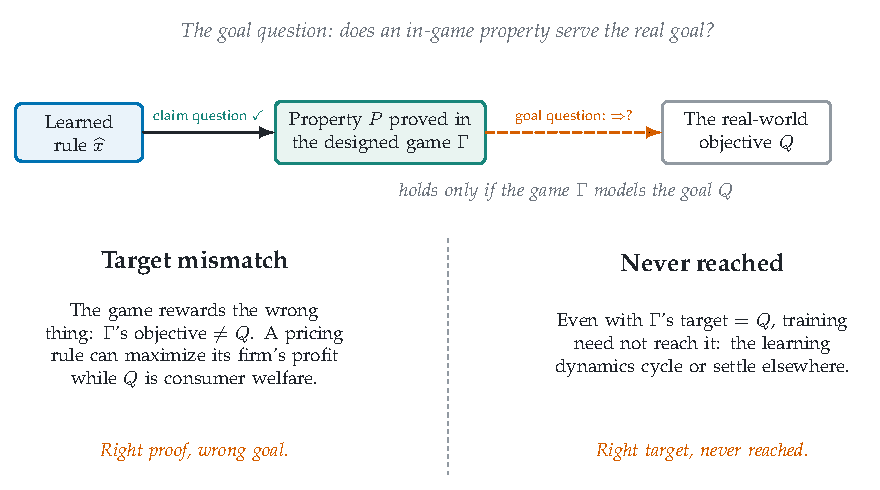
\includegraphics[width=\textwidth]{figure/fig6-goal-question.pdf}
\caption{The goal question. A designed game $\Gamma$ serves the real objective $Q$
only when its target property $P$ supports $Q$ and training reaches a policy with $P$.
The figure highlights two recurring failures: the game's target may fail to support $Q$
(\emph{target mismatch}), as when a pricing rule maximizes its firm's profit while $Q$
is consumer welfare; or the training dynamics may never reach the target even when the
two agree (\emph{never reached}). Both recur in training and oversight and in deployment governance
(\S\ref{sec:gt4ai:governance}); Section~\ref{sec:synthesis} states the same
composition in symbols.}
\label{fig:goal-question}
\end{figure}

\subsubsection{Preference games: what the aggregation certifies}

Preference learning starts from pairwise human comparisons (a person sees two model responses and
says which is better, the data behind RLHF), and must turn many such
comparisons into one policy. How it aggregates them is a design choice that changes the result. Collapsing
each response to a single score discards structure that keeping the
comparisons as a game would preserve. That choice in turn raises two
questions: whether the training converges, and which aggregation it is aiming
at.

Collapsing the comparisons into one hidden score per response, as a Bradley--Terry
model does, forces a straight-line ranking the comparisons need not
have~\citep{BradleyTerry1952}. Three responses can cycle, $A \succ B$, $B \succ C$,
and yet $C \succ A$ --- the rock-paper-scissors pattern again --- as they genuinely do
in psychological, social-choice, and online-comparison
settings~\citep{May1954,Tversky1969,Dudik2015}. A single score cannot represent a
cycle, so an approach built on one loses the cyclic part of the data.

A preference game keeps the comparisons intact and aggregates them through an
equilibrium instead. Nash learning from human feedback (NLHF) takes this route: it reads the
comparison model as a symmetric two-player game and looks for its equilibrium.
It adds one thing, a penalty for drifting too far from the starting policy,
measured in Kullback--Leibler (KL) divergence~\citep{Munos2024}. In plain
terms, the training procedure (Nash-MD) settles on the policy that best answers the
comparisons while staying close to where it began. Because the target rewards staying
near the start, a rival policy can win on the raw comparisons and still lose on the
penalized objective the game actually optimizes.

Whether that training actually reaches the equilibrium is a separate question. Without
such a penalty, in a plain zero-sum
preference game, common update rules can converge only on average while the current policy keeps cycling~\citep{Mertikopoulos2018}: the same
non-transitivity from Section~\ref{sec:gt4ai:evaluation}, now inside training. Building the penalty into the
payoff gives Nash-MD a last-iterate guarantee: in the tabular regularized setting
analyzed by \citet{Munos2024}, the current policy converges at an $O(1/T)$ rate.
Optimistic mirror descent and the extragradient method provide other last-iterate
results under their own game and algorithmic assumptions~\citep{Mertikopoulos2019}.
A convergence claim must specify the game, update rule, and sense of convergence.

Beyond convergence, the methods differ in what they aim at. Some keep this equilibrium
target and only change the optimizer: INPO (iterative Nash policy optimization) folds
no-regret self-play into a single loss, and DNO (direct Nash optimization) uses an
iterative direct-preference update~\citep{Zhang2025INPO,Rosset2024DNO}. Others change the target itself. SPO (self-play preference optimization)
adopts the Minimax Winner from social choice, the response whose worst
pairwise defeat is smallest. It builds cases where the standard reward-based
pipelines, RLHF and direct preference optimization (DPO), fail to recover
it~\citep{Swamy2024SPO}. Its experiments are in continuous control, not LLM
fine-tuning, so that failure is not yet shown for language models. The target is the substantive choice: a Minimax
Winner and a regularized Nash equilibrium turn the same comparisons into different
answers, and no amount of optimization skill decides which answer is the right one.

\subsubsection{Interactive-proof games: what a bounded judge can establish}

The second design depends on a specific asymmetry: a weak judge may be unable to follow
a whole proof yet still able to check one disputed step of it. Debate exploits that gap by
having two provers argue until the dispute narrows to a single step the judge can
actually rule on. Prover--Verifier Games work the same asymmetry from the prover's
side, training the prover to produce reasoning a weaker verifier can check.
Recursive reward modeling, iterated amplification, and process supervision
pursue the same oversight goal through other decompositions. Whether such a game is worth its complexity depends on three things. The
argument must let a limited judge reach conclusions it could not check alone,
it must reward honesty over manipulation, and it must help real judges and not
only idealized ones.

\runin{Formal motivation.} Complexity theory says why an exchange can add power. On its own, a limited judge can
check only claims that come with a short, quickly verifiable certificate: the class \textsc{NP}. Let two provers argue instead, over several back-and-forth rounds, and the
same polynomial-time judge can settle much harder questions. With optimal play
the reachable class is \textsc{Pspace}, the problems solvable with a
polynomial amount of memory, believed to be far larger than
\textsc{NP}~\citep{Irving2018}. The gain comes
from the interaction, not from the judge growing stronger. One subtlety is why debate
uses \emph{two} competing provers rather than one. A single-prover interactive proof lets the verifier run the checks for itself,
which is the \textsc{IP}$=$\textsc{Pspace} result, with \textsc{IP} the class
a randomized polynomial-time verifier can settle. In debate the human judge can
only be consulted as a black box, so the protocol relies instead on a second prover
with an incentive to contest an unsupported step, which leaves the judge to rule
only on a step that has been disputed. These are results about idealized provers and
a formal verifier under optimal play. They motivate the design and bound what such a
protocol could achieve in principle; whether a real judge is more accurate under it
is a separate, empirical question, taken up below.

\runin{Protocol design and assumptions.} The power is not automatic; it depends on who speaks when. \citet{Anil2021} show that if the prover moves first, an optimal prover can
remove all information from its message about the true answer. A protocol
where the verifier commits first restores the guarantees, and a simultaneous
version can settle into the judge simply ignoring the prover. This failure is \emph{information suppression}: the prover withholds the
telling detail rather than overwhelming the judge with evidence.

Even with the right turn order, honesty must be made cheap enough to win.
\citet{Kirchner2024} turn checkability into a training objective, teaching LLM provers
to produce reasoning weaker verifiers can assess, and observe a legibility tax: gains
in checkability can come with lower answer accuracy than correctness-only training. A
sharper problem arises when a wrong argument is easy to state but expensive to
refute~\citep{BarnesChristiano2020}. Doubly-efficient debate bounds the cost on both sides under a restricted
problem model. The honest strategy uses only polynomially more computation
than solving the task, and the verifier makes a fixed number of human-judgment
queries~\citep{BrownCohen2023}, given a human-verifiable record of polynomial
length (with extra conditions in the stochastic case). Prover--estimator
debate targets this information-hiding more directly, giving the honest participant, under
stability assumptions, a strategy about as cheap to run as its
opponent's~\citep{BrownCohen2025ProverEstimator}.

\runin{Evidence with human judges.} Whether any of this helps a real judge is an empirical question.
\citet{Khan2024} vary how strong the debaters are and find that stronger debaters
improve both model and human judges on difficult reading-comprehension questions. The
revealing comparison is with \emph{consultancy}, where a single advocate argues one
side and no one answers back: making that lone advocate more persuasive lowers judge
accuracy, whereas letting two opposed debaters compete raises it. Other studies are less optimistic. \citet{Parrish2022} find single-turn debate-style explanations do not improve
human accuracy in their setting. Across a wider task set, \citet{Kenton2024}
find debate consistently beats that one-sided consultancy, though its
advantage over plain question-answering shows up mainly on
reading-comprehension tasks where the debaters can see a passage the judge
cannot. Across these studies the advantage appears where the judge benefits from
information the interaction reveals and the task admits a useful decomposition; they
do not establish that it holds generally.

Both designs remain limited by what the judge can observe and verify, and both
carry a cost: population methods must train and maintain several
models, and preference self-play and debate add repeated generations and judge
calls. The real question is whether the gain in coverage or checkability is
worth the extra computation. In markets and delegation chains, finally, the interaction is no longer a
training component for one model but an external institution shared by many autonomous
actors.


\subsection{Deployment Governance: From Local Objectives to System Outcomes}
\label{sec:gt4ai:governance}

Once the game is a deployed institution rather than a designed training component ---
the last of the four objects --- no single participant owns the result. Each agent can implement its principal's objective
faithfully, and the system they jointly produce can still be one no principal asked
for. Algorithmic pricing makes this concrete. Even when every pricing agent
maximizes its own firm's profit and adapts well to its rivals, their interaction can
sustain supra-competitive prices and cut consumer surplus, with no individual
principal--agent relationship having failed. The failure is visible only when the
locally successful agents are evaluated together.

Two levers act on such a system, and they act at different moments. Before
deployment, a designer can alter the rules by which agents learn and the information
they see. After deployment, an auditor can test the behavior that actually occurred.
Both have been proposed for pricing. Recent work uses seller data to build
statistical tests of algorithmic pricing and states conditions under which an
algorithm passes~\citep{HartlineLongZhang2024,HartlineWangZhang2025}, while
\citet{Harrington2018} separately proposes making collusion by autonomous pricing
agents unlawful. In each case, the audit or the legal standard fixes the
alternatives a seller is compared against and the burden of proof it carries. That
choice, in turn, dictates what data must be collected.

The rest follows the dependencies among these choices. The objective and the affected
parties come first, because they fix what would count as a failure: in pricing,
consumers sit outside every principal--agent pair and still absorb the harm. The
objective then constrains the two levers, how the algorithm updates, fixed before
deployment, and which deviations an audit tests, applied after it. The lever chosen
fixes what the audit record must contain, down to the randomization a seller must
log. And the record fixes the scope of the inference it supports, from one seller's
conduct to a claim about the market.

\subsubsection{System objective and affected parties}
Naming the objective is harder than it sounds, because the natural accounting leaves
parties out. A local equilibrium or regret guarantee states a property that holds
inside the interaction as specified. Extending it to a claim about the system takes a
separate argument: who is affected, and what the institution is for. Delegation
games place that gap inside the principal--agent relation. \citet{Sourbut2024} separate two ways this can go wrong. A control failure is an
agent not doing what its principal wanted. A cooperation failure is agents interacting
badly even though each serves its own principal well. Both decompose into alignment and
capability components, with principal welfare as the evaluative object. Because principal welfare depends on collective
cooperation as well as on individual control, a property proved for one
principal--agent pair says nothing about the collective half.

Pricing adds a party the accounting misses entirely. Consumers are not principals in
the delegation game, so no term in it tracks what happens to them. Coordination among
profit-aligned pricing agents can therefore be a cooperation success by that measure
and a system failure the moment consumer welfare enters the objective. Deciding whose
outcomes count is thus a prior step rather than a detail of implementation: it fixes
which of those two readings the same behavior receives.

\subsubsection{Ex ante design of learning and information}
With the objective fixed, the earlier lever chooses how the agent learns and what it
is allowed to see. The algorithmic-pricing literature shows how much rides on that
choice. \citet{Calvano2020} find that Q-learning agents in repeated Bertrand
competition with differentiated products learn supra-competitive prices without any
direct communication. The learned strategies show punishment phases followed by a return to high prices, though the analysis proves no general
convergence theorem for Q-learning. \citet{Asker2022} isolate one source of this sensitivity: how the
algorithm updates. With no weight on future profits, synchronous updating, which computes returns for every price and not just the
one chosen, yields competitive prices in their baseline, whereas asynchronous updating can push prices near the
monopoly level. Once future profits carry positive weight, even synchronous updating
permits supra-competitive prices, though still less than asynchronous.
\citet{BanchioSkrzypacz2022} find the same sensitivity in what agents are told rather
than in how they update. In a repeated auction with two bidders of equal normalized
value and a discrete bid grid, first-price auctions sustain bids below the competitive
benchmark when bidders receive no extra feedback; revealing the lowest winning bid
raises competitiveness.

Theory and field evidence bear on the same sensitivity. \citet{Cartea2025} prove a
Folk-theorem-style result for boundedly rational learners using finite-memory
strategies in repeated potential games, a restricted class that does not transfer
directly to general differentiated Bertrand competition.
\citet{FishGonczarowskiShorrer2024} study LLM agents in place of hand-built learners:
their oligopoly experiments reach supra-competitive prices quickly and autonomously,
and seemingly innocuous changes to the prompt alter how far prices rise.
\citet{Assad2024} supply field evidence from German retail gasoline markets that are
not monopolies. Using headquarters-level adoption as an instrument, they estimate that
algorithmic pricing raises margins, with margins rising in duopoly and triopoly
markets once all competing stations adopt. The lesson for governance is direct: the
``algorithm'' label alone does not fix the market behavior to be evaluated. The update
rule and the information feed are what an ex ante standard would have to specify, and
an audit after the fact tests something different, namely whether the behavior
a deployment actually produced meets a standard.

\subsubsection{Ex post standards and deviation classes}
An audit tests behavior against alternatives the auditor names, so a standard is only
as strong as the set of alternatives behind it. That set is the deviation class. The choice among
classes settles three things in turn: what a passing seller has actually ruled out,
what a market of passing sellers collectively satisfies, and whether an algorithm can
pass the test while still doing harm.

The classes differ in how much a hypothetical deviator is allowed to change. External
regret compares realized profit against what one fixed price, used in every round,
would have earned. Internal regret asks a narrower question: would replacing one
chosen action $i$ by another $j$ have paid? Swap regret allows a separate replacement
for every chosen action. Calibrated regret is the version of swap regret written for
posted prices. For a finite price set $\mathcal{P}$, it is the largest average gain
available from any remapping $\sigma:\mathcal{P}\rightarrow\mathcal{P}$ that replaces
each posted price $p$ by $\sigma(p)$, holding that round's demand environment
fixed~\citep{HartlineLongZhang2024}. A seller with low calibrated regret has therefore
ruled out every profitable price-contingent remapping, a strictly finer test than
fixed-price deviations.

Passing that test everywhere supports a market-level statement, but a limited one. When
every player has vanishing internal regret, the empirical distribution of joint
actions approaches the set of correlated equilibria of the stage
game~\citep{FosterVohra1997,HartMasColell2000,BlumMansour2007}. That theorem
constrains conditional incentives in the observed distribution and nothing else. It
carries no welfare criterion and no legal one, so calling the resulting distribution
``competitive'' takes a benchmark the theorem does not supply.

\citet{HartlineLongZhang2024} supply one, defining unilateral non-collusion through
calibrated best response: conditional on whatever a seller's own price reveals, that
price must approximately maximize its expected profit in the demand environment that
price induces. The conditioning is essential, because the pattern of posted prices can
itself be information a seller acts on. Low calibrated regret is the dynamic version
of this condition, measured over a deployment history, and when every seller meets it
the joint price distribution forms a correlated equilibrium of the stage pricing game.
\citet{Hartline2026} then designates stage-game equilibrium prices as competitive and
the additional repeated-game equilibria as non-competitive. That gives the deviation
condition a concrete, usable meaning, while leaving the market assumptions and the welfare or legal benchmark as separate inputs. The correlated-equilibrium
result itself still implies nothing about consumer surplus.

Changing the deviation class changes which harmful behaviors can pass the test.
\citet{Braverman2018} exhibit a seller facing a buyer who runs EXP3, or any other
algorithm that responds to average past payoffs, and show the seller can extract
nearly the buyer's full welfare. The same paper builds a different no-regret algorithm
for the buyer, against which the seller can do no better than repeatedly posting the
Myerson reserve. Both buyer algorithms are no-regret by the same external standard;
the losses they expose the buyer to differ sharply.
\citet{HartlineWangZhang2025} make a matching point on the seller side, showing that
algorithms satisfying only best-in-hindsight regret can be driven to post
supra-competitive prices even when neither seller has side information.

External regret misses all of this because it compares the whole realized sequence
against a single fixed action. A profitable deviation can be conditional instead ---
replace price $p$ by $q$, but only in the rounds where $p$ was posted --- with no
single fixed price improving the average. Calibrated regret tests exactly those
price-contingent replacements, and a seller can satisfy it on its own, whatever its
rivals do.

\subsubsection{Auditability from deployment records}
Having the right test is not the same as being able to run it. Calibrated regret asks
what a seller would have earned at prices it did not post, and no record contains that
directly. \citet{HartlineLongZhang2024} recover it from a deployment log that keeps
three things per round: the price posted, the demand realized at that price, and the
distribution the seller drew that price from. Because the seller sometimes prices at
random, rarely posted prices still appear in the log, and demand at them can be
estimated by weighting the observed rounds by how likely each price was: the
inverse-propensity construction. The rarer a price, the more rounds it takes
to identify, so the data requirement grows as the smallest probability the algorithm assigns
to any price shrinks.

That gives a seller something to act on: deliberately adding exploration and logging
makes a competitive deployment auditable. The estimator needs no access to source
code, only credible internal records of the randomization and the outcomes, a logged
black-box audit whose validity rests entirely on the provenance and integrity
of the transcript.

An incomplete record yields a bound rather than a verdict. Pessimistic calibrated
regret drops the requirement that every price be posted with positive
probability~\citep{HartlineWangZhang2025}: where the transcript leaves a
counterfactual outcome unidentified, it reports the highest calibrated regret
consistent with any completion of the missing data. A low pessimistic value certifies
low regret under every compatible completion. A high value is ambiguous by construction: it may signal a real profitable
deviation, or only a record too thin to rule one out. The authors read a failure to supply a
low-regret certificate as violating a proposed per se rule, which places the
evidentiary burden on the seller. That is a legal choice, not a statistical one.

Unknown costs draw a second boundary of a different kind. Regret is computed from
profit, profit requires marginal cost, and the auditor rarely knows it. Suppose the auditor
lets marginal cost lie anywhere in a set $\mathcal{C}$. A seller then passes the
plausible-non-collusion test as soon as some $c\in\mathcal{C}$ makes its observed
behavior look low-regret, even when the true cost would imply high regret. A high
assumed cost can thus rationalize supra-competitive prices that were in fact generated
at a lower one, and the wider $\mathcal{C}$ is, the weaker the test becomes. How wide
it may be is set by the cost evidence available and by the governing legal standard,
not by the data alone.

\subsubsection{From individual evidence to market-level conclusions}
A clean audit of one seller remains a statement about that seller. Getting from there
to a claim about the market is not automatic, and the gap has been made explicit.
\citet{Arunachaleswaran2025} study sequential deployment: the first seller commits to
any no-regret algorithm, and the second then optimizes against the environment that
commitment creates. Supra-competitive prices arise whenever the second seller earns at least what random pricing would earn, including when its choices are
restricted to price distributions that ignore what the first seller does. They also construct an
equilibrium in algorithm space with near-monopoly prices and no threats written into
either algorithm. \citet{HartlineClarification2026} classifies that outcome as
non-competitive while declining to call it collusion. One seller learns a best
response; the other uses the non-competitive static strategy. The outcome violates the
stage-game competitive benchmark, yet the evidence is not enough to show that the two
acted jointly.

The lesson is about scope. Low calibrated regret is a property of an individual
seller; the correlated-equilibrium conclusion is a property of the market, and it
follows only when \emph{every} seller has it. Let one seller fail and the market-level
conclusion is gone. Whether antitrust law should prohibit high-regret or naively
non-optimizing pricing when no agreement is proven is a policy question, and a failed
audit by itself does not establish an agreement among
sellers~\citep{Harrington2018}.

The two levers, then, act at different times and answer different questions. Design
before deployment changes the update rule or the information structure; auditing after
it evaluates the behavior that resulted. When every seller has low calibrated regret,
the data do impose a stage-game equilibrium restriction on the market outcome. That
restriction answers the claim question and leaves the goal question open: whether the
market it describes is one a regulator should accept. Answering it takes an explicit objective for each
agent and a separate criterion for the market. A seller can optimize the objective it
was assigned even when the market it helps produce fails the criterion that matters.

% conclusion.tex
% Section 5: Synthesis and Outlook

\section{Synthesis and Outlook}
\label{sec:synthesis}

\subsection{Combining Output and System Validity}
\label{sec:synthesis:compose}

Output validity is a claim about the learned object itself. System validity
connects a result obtained in a designed game to the objective outside that
game:
\[
\begin{aligned}
\text{output validity:}\qquad
&\widehat{x} \quad\Longrightarrow?\quad P_\Gamma(\widehat{x}),\\
\text{system validity:}\qquad
&P_{\Gamma_Q}(x) \quad\Longrightarrow?\quad Q(x),
\end{aligned}
\]
where $\Longrightarrow?$ marks an implication whose validity is the object of
study, $P_\Gamma$ is a property defined for a game $\Gamma$, and $Q$ is the
objective around which $\Gamma_Q$ was designed.

Composition requires the same object, game, and domain in both claims. Setting
$x=\widehat{x}$ and $\Gamma=\Gamma_Q$ gives
\[
\widehat{x} \;\Longrightarrow\; P_{\Gamma_Q}(\widehat{x}) \;\Longrightarrow\;
Q(\widehat{x}).
\]
Algorithmic pricing illustrates why the conditions matter. Each pricing
algorithm may satisfy a local criterion while the market fails an external
welfare objective. The local property concerns one firm maximizing its own
profit. The system objective concerns the joint market outcome and includes
consumers who are affected parties outside that local optimization.

For an output property defined through deviations, finite search generally
provides a lower bound on the largest gain. Assume that the target class contains
a null deviation, and define
$g_\Gamma(x)=\sup_{d\in\mathcal{D}_\Gamma(x)}\Delta_\Gamma(x,d)$ as the largest
gain over that class. A search that returns some $\widehat d$ establishes the
lower bound $g_\Gamma(x)\ge\Delta_\Gamma(x,\widehat d)$.
An upper bound on $g_\Gamma$ requires a guarantee on the search itself: if
$\Delta_\Gamma(x,\widehat d)\ge g_\Gamma(x)-\epsilon$, then observing
$\Delta_\Gamma(x,\widehat d)\le\eta$ yields $g_\Gamma(x)\le\eta+\epsilon$.
Without such a guarantee, the observation controls only the searched class.
Figure~\ref{fig:candidate-counterexample} summarizes this asymmetry between
finite counterexample search and a claim over the full deviation class.

Identification claims instead use observations and maintained assumptions to
define an identified set. They need not involve a searched deviation class.

\begin{figure}[pos=h]
\centering
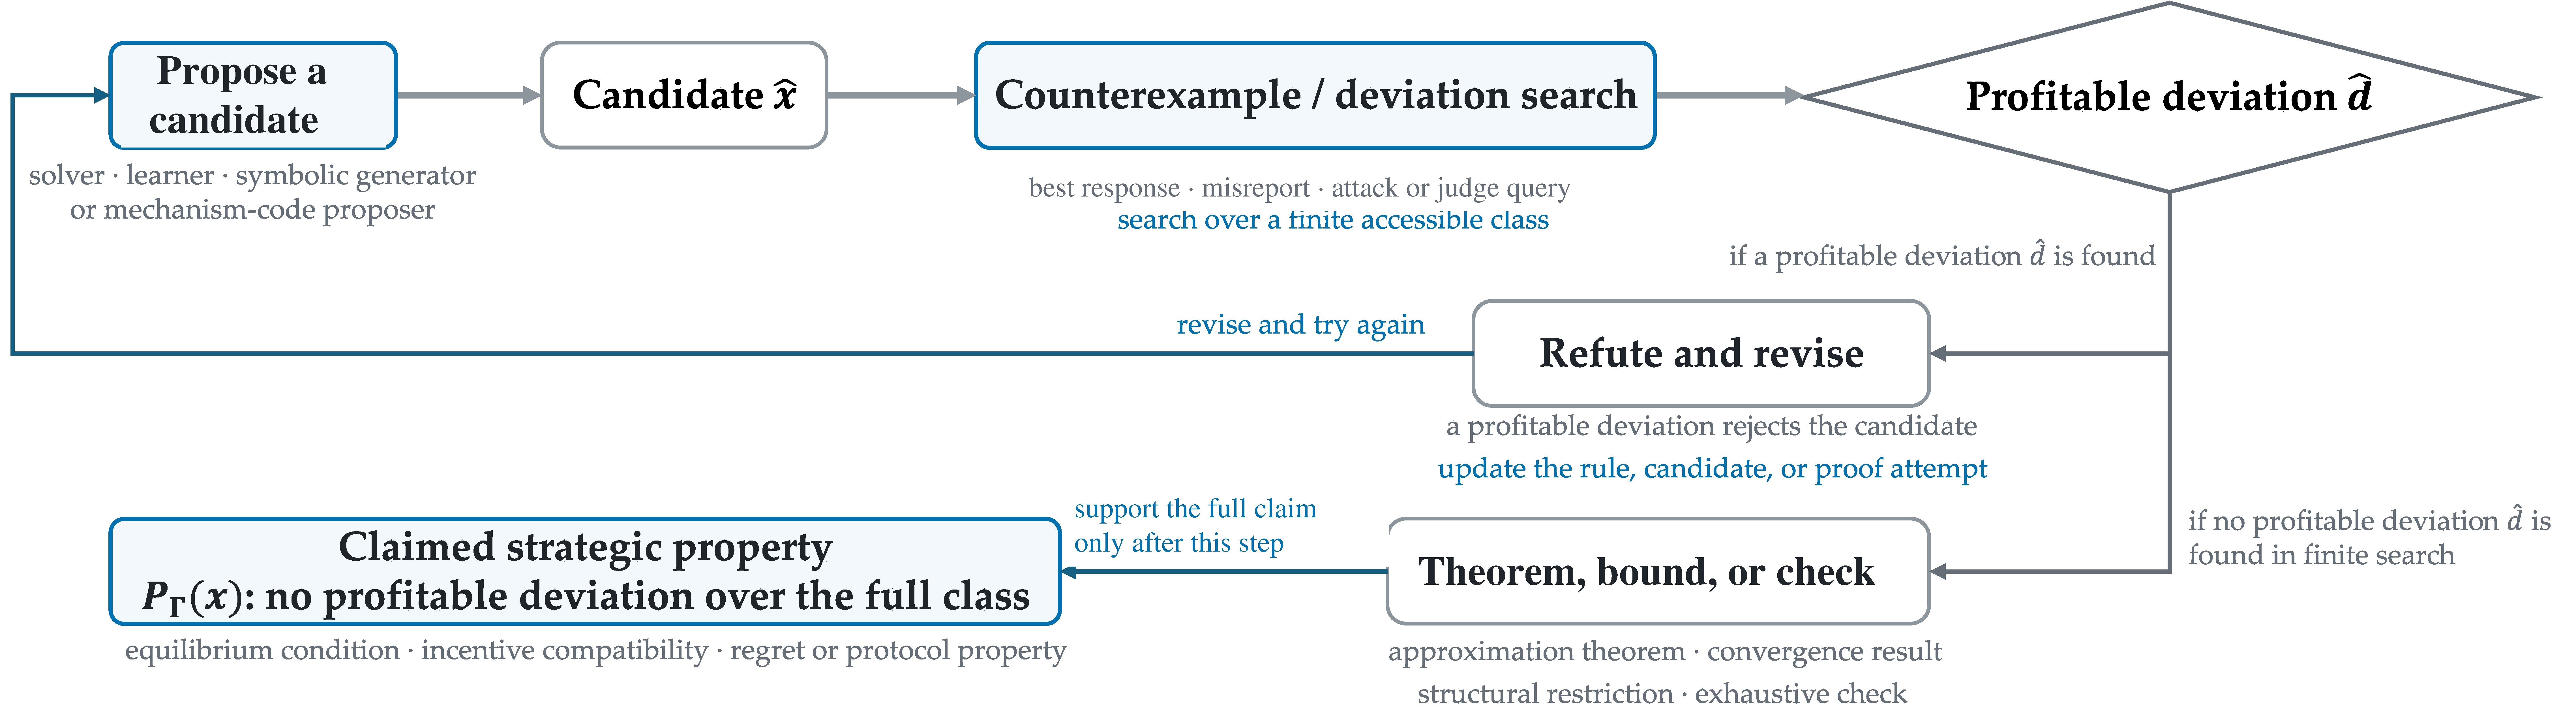
\includegraphics[width=\textwidth]{figure/fig4-candidate-counterexample.pdf}
\caption{Finite evaluation of a deviation-defined property. A method proposes a
candidate and searches for a profitable deviation in an accessible class. A
discovered deviation refutes the candidate. If the search finds none, a claim
over the target class requires a theorem, bound, or structural argument that
controls the alternatives not searched. Identification and system-validity
claims require different arguments.}
\label{fig:candidate-counterexample}
\end{figure}

\subsection{What Each Domain Contributes}
\label{sec:synthesis:map}

Table~\ref{tab:domain-map} summarizes the primary limitation in each domain and
the additional argument needed for the target claim.

Broader search and response oracles address coverage, whereas identification
depends on new information or maintained restrictions. Cross-game variation,
exploration, and logging can reveal otherwise unobserved counterfactuals.
Pessimistic completion converts counterfactuals that remain unidentified into
conservative bounds.

\begin{table}[htbp]
\centering
\caption{The six domains, the question each makes concrete, and what connects
finite evidence to the target claim.}
\label{tab:domain-map}
\begin{tabularx}{\textwidth}{@{}p{2.6cm} p{2.1cm} p{2.0cm} Y@{}}
\toprule
\textbf{Domain} & \textbf{Question} & \textbf{Primary limit} & \textbf{Additional argument} \\
\midrule
Constructive equilibrium (\S\ref{sec:ai4gt:equilibrium})
& Output validity & Coverage
& Duality in the zero-sum case; the regret decomposition; safe-resolving bounds; an executable derivation \\
\addlinespace
Strategic inference (\S\ref{sec:ai4gt:inference})
& Output validity & Identification
& Falsifiability plus recoverability; cross-game and cross-environment variation; maintained restrictions \\
\addlinespace
Mechanism design (\S\ref{sec:ai4gt:mechanism})
& Output validity under response & Coverage
& Membership in a truthful family; post-processing with a regularity bound
carrying a finite grid to a continuous domain; a stated deployment-domain
argument where participation or reports shift \\
\addlinespace
Strategic evaluation (\S\ref{sec:gt4ai:evaluation})
& Output validity under response & Coverage
& Response-oracle expansion over a stated policy class, or a certified robustness radius \\
\addlinespace
Designed games as evidence (\S\ref{sec:gt4ai:training})
& System validity & Designed-game scope
& Protocol theorems with stated bounds on adversary and judge; an argument that the constructed objective is the intended one \\
\addlinespace
Deployment governance (\S\ref{sec:gt4ai:governance})
& System validity & Coverage \emph{and} identification
& Correlated-equilibrium restrictions from low calibrated regret; pessimistic completion; an external welfare or legal benchmark \\
\bottomrule
\end{tabularx}
\end{table}

\begin{table}[htbp]
\centering
\caption{Four forms of evidence used in the surveyed domains, together with the
claims and assumptions associated with each. A system may combine several
forms.}
\label{tab:strategic-evidence}
\footnotesize
\setlength{\tabcolsep}{3.5pt}
\renewcommand{\arraystretch}{1.25}

\begin{tabularx}{\textwidth}{
    >{\raggedright\arraybackslash}p{0.15\textwidth}
    >{\raggedright\arraybackslash}p{0.22\textwidth}
    Y
    Y
}
\toprule
\textbf{Evidence basis}
& \textbf{Claim supported}
& \textbf{Scope and assumptions}
& \textbf{Conclusion and cost}
\\
\midrule

Machine-checked derivation
& Equilibrium or approximation property of a strategy profile or synthesized
algorithm
& Explicit formal game or algorithm; sound encoding and trusted checker
& Deductive result for the encoded statement; construction and checking cost
\cite{PrimeNash2025,LegoNE2025}
\\

\addlinespace

Structural theorem
& Incentive compatibility or strategy-proofness of a mechanism
& Membership in the theorem's representation family; domain and regularity
assumptions
& Exact or bounded theorem-specific result; representation and post-processing
cost \cite{Shen2019,Duan2023,Duetting2024}
\\

\addlinespace

Protocol theorem
& Soundness, completeness, or a winning-strategy result for an interactive
protocol
& Specified roles and information; bounds on the judge, adversary, and available
computation
& Result within the protocol model; verifier resources
\cite{Irving2018,BrownCohen2023}
\\

\addlinespace

Behavioral statistical test
& Regret or another specified property of a deployed policy
& Logged play and assumptions on sampling, exploration, and the market
& Probabilistic result for the data-generating process; sample and computation
cost \cite{HartlineLongZhang2024,HartlineWangZhang2025}
\\
\bottomrule
\end{tabularx}
\end{table}
\FloatBarrier

\subsection{Research Priorities}
\label{sec:synthesis:open}

For each empirical estimate of strategic performance, reproducible comparisons
require authors to identify the alternative class and explain how it relates to
the target claim. Cost comparisons should report training and evaluation as
well as per-instance inference.

Strategic inference should make greater use of partial identification. When
several latent explanations fit observed play, the relevant question is which
counterfactual conclusions hold across the identified set. Pessimistic
completion in deployment auditing provides one example of this approach.

Claims about training and oversight protocols should state the modeled resource
and information bounds on every participant. These assumptions determine what
the designed game establishes and should appear in the main statement of the
result.

Deployment studies also need evaluation domains that account for participant
responses. This requires a model or audit of how those responses select the
post-deployment cases to which the property is claimed to extend.


\printcredits

\section*{Acknowledgments}

%% Loading bibliography style file
\bibliographystyle{cas-model2-names}

% Loading bibliography database
\bibliography{ref}

\end{document}
